%% BioMed_Central_Tex_Template_v1.06
%%                                      %
%  bmc_article.tex            ver: 1.06 %
%                                       %

%%IMPORTANT: do not delete the first line of this template
%%It must be present to enable the BMC Submission system to
%%recognise this template!!


%%% additional documentclass options:
%  [doublespacing]
%  [linenumbers]   - put the line numbers on margins

%%% loading packages, author definitions

%\documentclass[twocolumn]{bmcart}% uncomment this for twocolumn layout and comment line below
\documentclass{bmcart}

%%% Load packages
%\usepackage{amsthm,amsmath}
%\RequirePackage{natbib}
%\RequirePackage[authoryear]{natbib}% uncomment this for author-year bibliography
%\RequirePackage{hyperref}
\usepackage[utf8]{inputenc} %unicode support
\usepackage{algorithmic}
\usepackage{rotating}
\usepackage{amsmath}
\usepackage{multirow}
\usepackage{enumerate}
\usepackage{algorithm}
\usepackage{subfigure}
%\usepackage[applemac]{inputenc} %applemac support if unicode package fails
%\usepackage[latin1]{inputenc} %UNIX support if unicode package fails


%%%%%%%%%%%%%%%%%%%%%%%%%%%%%%%%%%%%%%%%%%%%%%%%%
%%                                             %%
%%  If you wish to display your graphics for   %%
%%  your own use using includegraphic or       %%
%%  includegraphics, then comment out the      %%
%%  following two lines of code.               %%
%%  NB: These line *must* be included when     %%
%%  submitting to BMC.                         %%
%%  All figure files must be submitted as      %%
%%  separate graphics through the BMC          %%
%%  submission process, not included in the    %%
%%  submitted article.                         %%
%%                                             %%
%%%%%%%%%%%%%%%%%%%%%%%%%%%%%%%%%%%%%%%%%%%%%%%%%

%\def\includegraphic{}
%\def\includegraphics{}

%%% Put your definitions there:
\startlocaldefs
\endlocaldefs



\begin{document}
\begin{frontmatter}
\begin{fmbox}
\dochead{Research}

\title{Improving the performance of relaxed clock model in phylogenetic analysis}

\author[
   %addressref={aff1},                   % id's of addresses, e.g. {aff1,aff2}
   %email={rzha419@aucklanduni.ac.nz}
]{\inits{}\fnm{Rong} \snm{Zhang}}
\author[
   addressref={aff1},
   corref={aff1},                       % id of corresponding address, if any
   email={alexei@cs.auckland.ac.nz}   % email address
   %noteref={n1},                        % id's of article notes, if any
]{\inits{}\fnm{Alexei} \snm{Drummond}}

\address[id=aff1]{%                           % unique id
  \orgname{Department of Computer Science, University of Auckland}, % university, etc
  \street{Princes Street},                     %
  \postcode{1010}                                % post or zip code
  \city{Auckland},                              % city
  \cny{New Zealand}                                    % country
}

%\address[id=aff2]{%
%  \orgname{},
%  \street{},
%  \postcode{}
%  \city{},
%  \cny{}
%}

%\begin{artnotes}
%%\note{Sample of title note}     % note to the article
%\note[id=n1]{Equal contributor} % note, connected to author
%\end{artnotes}

\end{fmbox}% comment this for two column layout

%%%%%%%%%%%%%%%%%%%%%%%%%%%%%%%%%%%%%%%%%%%%%%
%%                                          %%
%% The Abstract begins here                 %%
%%                                          %%
%% Please refer to the Instructions for     %%
%% authors on http://www.biomedcentral.com  %%
%% and include the section headings         %%
%% accordingly for your article type.       %%
%%                                          %%
%%%%%%%%%%%%%%%%%%%%%%%%%%%%%%%%%%%%%%%%%%%%%%
\begin{abstractbox}
\begin{abstract}
Bayesian MCMC plays an important role in phylogenetic analysis. However, due to the huge amount of phylogenetic data, the efficiency becomes a great problem. Based on uncorrelated relaxed clock model, this paper introduces a new operator to propose evolutionary rates and divergence times at the same time, under the condition that the genetic distances are constant. Specifically, the proposed operator deals with three rates when changing the node time for an internal node. For the root of a phylogenetic tree, there are three strategies discussed, including Simple Distance, Small Pulley and Big Pulley. It is noticed that Big Pulley is able to change the tree topology, which enables the operator to sample all the possible trees under an unrooted tree.  To validate the effectiveness, a series of experiments have been performed by implementing the proposed operator in BEAST2 software. The results prove that the proposed operator is able to improve the performance by giving better estimations and less running time. 
%%(quantitatively, ESS per hour!!!)
\end{abstract}

\begin{keyword}
\kwd{Bayesian MCMC}
\kwd{Operator}
\kwd{Phylogenetic trees}
\kwd{Genetic distances}
\kwd{Divergence times}
\kwd{Evolutionary rates}
\end{keyword}

% MSC classifications codes, if any
%\begin{keyword}[class=AMS]
%\kwd[Primary ]{}
%\kwd{}
%\kwd[; secondary ]{}
%\end{keyword}

\end{abstractbox}
%
%\end{fmbox}% uncomment this for twcolumn layout
\end{frontmatter}

%%%%%%%%%%%%%%%%%%%%%%%%%%%%%%%%%%%%%%%%%%%%%%
%%                                          %%
%% The Main Body begins here                %%
%%%%%%%%%%%%%%%%%%%%%%%%%%%%%%%%%%%%%%%%%%%%%%

%%%%%%%%%%%%%%%%
\section*{Introduction}
Phylogenetics has attracted much research interest over the years. More and more scientists are becoming keen to discover the evolutionary history of life, such as birds \cite{hackett2008phylogenomic}, primates \cite{szalay2013evolutionary}, grasses \cite{kellogg2001evolutionary} and so on \cite{sawabe2007inferring,garnery1992evolutionary}. One fundamental concept in phylogenetics is a graph model that shows the relationships among species and organisms, which is called a phylogenetic tree. The main task for phylogenetic analysis is aimed at inferring the phylogenies by constructing the phylogenetic trees. Until now, a lot of methods have already been proposed and a majority of them have been implemented in the computer softwares, such as BEAST2 \cite{drummond2007beast, bouckaert2014beast} , MRBAYES \cite{huelsenbeck2001mrbayes} and APE \cite{paradis2004ape}.

Traditional methods for constructing phylogenetic trees are based on a distance matrix that is obtained by sequence alignment, after biologists extract DNA from organisms. In the last few decades, more advanced techniques have been developed to reconstruct phylogenetic trees, due to the development of statistics and computer science. One popular research area called Bayesian phylogenetics puts an emphasis on a sampling process to construct the phylogenetic tree, in which the methods based on Markov Chain Monte Carlo (MCMC) provide a computational tool for sampling problems. Early in 1997, Yang and Rannala presented a Bayesian framework that includes the specified prior for phylogenies and ancestral speciation times, and the posterior probabilities of phylogenies to be inferred as the maximum posterior probability (MAP) tree \cite{yang1997bayesian}. By virtue of a sampling method, a set of trees with probabilities is obtained, so that Monte Carlo integration can be used to integrate over the ancestral speciation times for particular trees. Based on this framework, much attention has been paid to estimating the divergence times \cite{rannala2003bayes,yang2003comparison,reis2011approximate}.
%%more details about the Bayesian work

For phylogenetic analysis based on Bayesian MCMC, the efficiency of a sampling method is always the main issue that should be carefully handled. In particular, the calculation of the phylogenetic likelihood is a large burden of the efficiency. Hence, some researchers have tried to improve the likelihood calculations, such as detection of repeating sites \cite{kobert2017efficient}. On the other hand, in MCMC methods, the operators that propose a new state based on the current state also have a leading influence on the overall performance. As is discussed by Lakner et al., the major limitation in Bayesian MCMC analysis of phylogeny lies in the efficiency with which operators sample the tree space \cite{lakner2008efficiency}. So far, there have been already many different kinds of operators proposed. According to the work in Ref. \cite{hohna2011guided}, the two common operators, i.e. prune-and-regraft and subtree-swap, both contribute to a tree with low likelihood since they propose a new tree by random movement of the current tree. So the authors introduced two new operators by proposing a state from a discrete set of possible proposals and narrowing the proposal distribution to the more likely proposals. Their experimental results proved that the two operator have faster average run time and more accurate predictability.

Nevertheless, it is acknowledged that a faster and more reliable performance is also dependent on a good mixture of operators and different operators may be applicable for different objects. In this paper, a novel operator is proposed in the case where genetic distances are constant. Namely, the proposed operator is used to change the divergence times of nodes and evolutionary rates on the branches at the same time without changing the genetic distances, so that the likelihood of the phylogenetic tree remains unchanged. In addition, the proposed operator has been implemented as a new package in BEAST2 software. After a series of simulations and experiments, the results prove that the proposed operator can provide correct samples  and work properly in Bayesian phylogenetic analysis. According to the comparisons, it is concluded that by using the proposed operator, the efficiency of sampling parameters can be increased by.%%mention the ESS per hour

The following of this paper is constructed as follows: Section 2 gives some preliminary theories of the work related to this paper. Section 3 introduces the proposed operator, which includes the mechanism for internal nodes and 3 different strategies for the root. The experiments and discussions are detailed in the 4th section to validate the efficiency of the proposed operator. Section 5 ends the paper with a short conclusion.
\section*{Prelimiaries}
\subsection*{Bayesian MCMC}
Eq.(\ref{bayes}) shows a basic Bayesian framework for phylogenetic analysis. It consists of prior distributions for the tree $g$ and a set of parameters of interest $\Phi $, a phylogenetic likelihood that conveys information from data $D$, and the posterior distribution to be inferred, which is denoted in the form of probability density by $p(g) $, $p(\Phi )$, $p(D|g,\Phi )$, $f(g,\Phi |D)$ correspondingly. From a Bayesian perspective, the biological data, phylogenetic trees and the parameters in the model exist with some probabilities and are related by the Bayes' formula. As a result, it is able to jointly infer evolutionary history of species with various models that describe the evolutionary process.
%%construct the Bayes equation for our model after this section
\begin{eqnarray}\label{bayes}
p(g,\Phi |D) = \frac{{p (D|g,\Phi ) \times p (g) \times p (\Phi )}}{{p (D)}}
\end{eqnarray}

On the other hand, due to the huge amount of data and the marginal likelihood being difficulty to calculate, Markov Chain Monte Carlo (MCMC) algorithms are adopted to get samples from the posterior distribution. 
%%introduce what is MCMC, and the method of MH-MCMC?
\subsection*{Tree proposals}
\label{treeproposals}
The term ``operator" used in this paper is defined as the tree proposal in Bayesian phylogenetics, and is used to propose a new state that is only dependent on the current state.

For now, there are some classical and frequently-used operators, such as a random walk operator which proposes a new state by adding a random number, and a scale operator which multiplies the current state with a scale factor. But they are suitable for working on a single parameter or a set of parameters, such as population size. To make a proposal about the tree topology, it is also necessary to include other operators, such as subtree slide operator, swap operator, narrow operator and so on. On top of this, there are also some extended operators available to help give the better performance. For instance, the prune-and-regraft operator selects a random subtree and reattaches the subtree at a new random branch. And the subtree-swap operator exchanges two random subtended subtrees. 
%%cite some papers of using the operator

What matters for developing an operator is that the proposal should be reversible. As is discussed in Green's paper \cite{green1995reversible}, the constructed Markov transition kernel $P(x,dx')$ should satisfy the detailed balance, as is represented by Eq.(\ref{balance}). In other words, the probability that the operator propose a new state from the current state is required to be equal to the probability that the proposed state goes back to current state. Therefore, as is shown in Eq.(\ref{Ratio}), to ensure the detailed balance in the MCMC chain, a ratio ${q(x',dx)}/{q(x,dx')}$ should always be included in the probability $\alpha(x,x')$ that the proposal made by the operator is accepted.
\begin{equation}\label{balance}
\int_A {\int_B {\pi (dx)P(x,dx')} }  = \int_B {\int_A {\pi (dx')P(x',dx)} }
\end{equation}
, where ${\pi (dx)}$ is the target distribution, $A$ and $B$ are Borel sets in parameter space $\varphi$.
\begin{equation}\label{Ratio}
{\alpha}(x,x') = \min \left\{ {1,\frac{{\pi (dx'){q}(x',dx)}}{{\pi (dx){q}(x,dx')}}} \right\}
\end{equation}
, where $x$ $x'$ $dx$ $dx'$.The ratio ${q(x',dx)}/{q(x,dx')}$ is called Hasgtings ratio.
%%explain the parameter and p or q!
%%pay attention to the Jacobian matrix below, explain why need to calculate
\subsection*{Uncorrelated relaxed clock model}
A clock model is used to model how rates evolve along branches in the phylogenetic tree, so that a time tree can reconcile with the genetic distances between sequences described by a substitution model. For example, a strict clock model assumes evolution rates to be the same at every branch. However, a relaxed clock model allows rates to vary across lineages so that better estimates of divergence times can be obtained. As a incomplete way of relaxing, a random local clock model only allows rates to be different within a subregion of the tree. 
%%cite paper

This paper is aimed at improving the performance of relaxed clock model in Bayesian phylogenetic analysis. The proposed operator is based on an uncorrelated relaxed model, where the rates vary and follow a certain distribution. As is detailed in Ref.\cite{drummond2006relaxed}, uncorrelated rates indicate that the rate on each branch is identically distributed and will be independently drawn from a certain distribution such as a log-normal distribution. As a result, the rates can change faster than making a slight move over multiple adjoining branches.
%%write the equation for inferring models Bayes!
\section*{The proposed operator}
In this section, we define the proposed operator as ConstantDistance Operator. Fig.\ref{flowchart} illustrates the flow chart of the proposed operator. In a phylogenetic tree, the node to operate on is denoted by \textbf{X}. And the proposed operator works differently on the internal nodes and the root of the tree. The details of the operations are introduced step by step in the following subsections.
\subsection*{The internal node operator}
Fig.\ref{internalnodes} represents the tree (or subtree of a phylogenetic tree) with the node \textbf{X} that is randomly selected among the internal nodes. The original tree in the current state is denoted by $g_{in}$. And the following 5 steps will propose a new tree ${g_{in}}'$.

\emph{Step 1} Get the parent node and two child nodes of \textbf{X}, denoted by \textbf{P}, \textbf{Ch1} and \textbf{Ch2} respectively.

\emph{Step 2} Get the nodes times of \textbf{X}, \textbf{P}, \textbf{Ch1} and \textbf{Ch2} , denoted by $t_X$, $t_P$, $t_1$, $t_2$, as well as the rates on the branches above the nodes, denoted by $r_i$, $r_j$, $r_k$.

\emph{Step 3} Propose a new node time for \textbf{X} by ${t_X}' = {t_X} + a$, where $a$ follows a Uniform distribution with a symmetric window size, i.e. $a \sim U[ - w, + w]$. Make sure that the proposed time is valid, i.e. $\max \{ {t_1},{t_2}\}  < {t_X}' < {t_P}$ holds.

\emph{Step 4} Propose new rates by using Eq.(\ref{int_rate}).
\begin{equation}
 \label{int_rate}
{r_i}' = \frac{{r_i} \times ({{t_P} - {t_X}})}{{{t_P} - {t_X}'}}\\
{r_j}' = \frac{{{r_j} \times ({{t_X} - {t_1}})}}{{{t_X}' - {t_1}}}\\
{r_k}' = \frac{{{r_k} \times ({{t_X} - {t_2}})}}{{{t_X}' - {t_2}}}
 \end{equation}

\emph{Step 5} Return the Hastings ratio.
\subsection*{The root operator}
For the root of the tree, there are three strategies to propose the new rates and node times. To be more specific, Simple Distance is a way of proposing a new root time only. Considering the genetic distance, Small Pulley adjusts the distances of branches on each side of the root. Moreover, under the constraint that the unrooted tree is fixed, Big Pulley proposes a new tree topology by rearranging the root.  Details are discussed below
\subsubsection*{Simple Distance}
Fig.\ref{simpledistance} shows the trees that are rooted at the node $X$. The original tree in the current state is shown in Fig.\ref{simpledistance}(a), which is denoted by $g_r$. Inspired by the operations on internal nodes, we will use the following steps to propose a new tree ${g_{r1}}'$, and keep the genetic distances $d_i$ and $d_x$ constant at the same time, as is illustrated in Fig.\ref{simpledistance}(b).

\emph{Step 1} Get the child nodes of the root \textbf{X}, denoted by \textbf{son} and \textbf{dau}. Their corresponding node times and rates are $t_X$, $t_j$, $t_k$ and $r_i$, $r_x$.

\emph{Step 2} Propose a new node time for the root \textbf{X} by \textbf{X} by ${t_X}' = {t_X} + a$, where $a \sim U[ - w, + w]$. Make sure that ${t_X}' > \max \{ {t_j},{t_k}\} $ holds.

\emph{Step 3} Propose new rates for branches on each side of the root by using Eq.(\ref{sim_rate}).
\begin{equation}
\label{sim_rate}
{r_i}' = \frac{{{r_i} \times ({{t_X} - {t_j}})}}{{{t_X}' - {t_j}}}\\
{r_x}' = \frac{{{r_x} \times ({{t_X} - {t_k}})}}{{{t_X}' - {t_k}}}
 \end{equation}

\emph{Step 4} Return the Hastings ratio.
\subsubsection*{Small Pulley}
Different from Simple Distance, a new genetic distance of branch on one side of the root is proposed in Small Pulley. As is illustrated in Fig.\ref{simpledistance}, Small Pulley proposes a new tree ${g_{r1}}'$ in Fig.\ref{simpledistance}(c), based on the original tree $g_r$ in Fig.\ref{simpledistance}(a). In order to maintain the total genetic distance of $d_i$ and $d_x$ unchanged, once ${d_i}'$ is proposed, $d_x$ will be adjusted by ${d_x}'$ simultaneously. The detailed process includes the following 4 steps.

\emph{Step 1} Get the child nodes of the root \textbf{X}, denoted by \textbf{son} and \textbf{dau}. Their corresponding node times and rates are $t_X$, $t_j$, $t_k$ and $r_i$, $r_x$. So the genetic distances can be calculated according to Eq.(\ref{sma1_dis}).
\begin{equation}
\label{sma1_dis}
{d_i} = {r_i} \times ({{t_X} - {t_j}})\\
{d_x} = {r_x} \times ({{t_X} - {t_k}})
 \end{equation}

\emph{Step 2} Propose a new genetic distance for $d_i$ by adding a random number that follows a Uniform distribution, i.e.  ${d_i}' = {d_i} + b$, where $b \sim U[ - v, + v]$. Make sure that $0 < {d_i}' < D$ holds, where $D = {d_i} + {d_x}$.

\emph{Step 3} Propose new rates for branches on each side of the root by using Eq.(\ref{sma1_rate}).
\begin{equation}
\label{sma1_rate}
{r_i}' = \frac{{{d_i}'}}{{{t_X} - {t_j}}}\\
{r_x}' = \frac{{D - {d_i}'}}{{{t_X} - {t_k}}}
 \end{equation}

\emph{Step 4} Return the Hastings ratio.
\subsubsection*{Big Pulley}
Big Pulley is used to sample the rates and times from a fixed unrooted tree so that the genetic distances among taxon are constant, which means the location of the root will be rearranged.

Firstly, a method called \textit{Exchange (Node1,Node2)} is designed to propose a new tree topology in this circumstances. to be specific, for the original tree $g$ in Fig.\ref{exchangemethod}, once the method \textit{Exchange (\textbf{B},\textbf{C})} is called, the following operations will be performed to proposed a new tree $g'$.
\begin{itemize}
\item Exchange the node \textbf{B} and \textbf{C} by pruning and grafting, i.e. cutting \textbf{B} (\textbf{C}) at its original position and attaching it to the original position of \textbf{C} (\textbf{B}).
\item Propose ${d_i}'$ by ${d_i}' = {d_i} + b$, where $b \sim U[ - v, + v]$. Make sure that $0 < {d_i}' < D$ holds, where $D = {d_i} + {d_x}$.
\item To maintain the genetic distances $d_{AB}$, $d_{AC}$ and $d_{BC}$ constant, the distances on the other three branches $d_j$, $d_k$ and $d_x$ will be adjusted by using Eq.(\ref{big_dis}).
% \begin{subequations}\label{big_dis}
%  \begin{equation}
%{d_j}' = {d_j}
%  \end{equation}
%  \begin{equation}
%{d_k}' = {d_k} - {d_i}'
%  \end{equation}
%    \begin{equation}
%{d_x}' = {d_x} + {d_i}
%  \end{equation}
%\end{subequations}
\begin{equation}\label{big_dis}
{d_j}' = {d_j}\\
{d_k}' = {d_k} - {d_i}'\\
{d_x}' = {d_x} + {d_i}
\end{equation}
\end{itemize}

As can be seen from the above descriptions, the method \textit{Exchange (Node1,Node2)} is actually aimed at swapping two nodes and reassigning distances on the four branches. That is to say, after using \textit{Exchange (\textbf{B},\textbf{C})}, the distances $d_i$, $d_j$, $d_k$ and $d_k$ will be adjusted to maintain the distances between node \textbf{A}, \textbf{B} and \textbf{C}, as the tree topology changes. 

Secondly, before applying this method in Big Pulley, there are two different tree shapes to take into consideration. In Fig.\ref{treeshape}, a symmetric tree is shown on the left, in which both the child nodes of the root have child nodes. But in the asymmetric tree on the right, only one of the child nodes of the root has child nodes below it, which means the other child node of the root is a leaf node. Hence, Big Pulley also differs when it works on a symmetric and asymmetric tree. The corresponding operations are detailed in the following two parts.
\paragraph*{Symmetric tree shape}

For the symmetric tree in Fig.\ref{treeshape}, the operations are illustrated in Fig.\ref{symmetric}, after which one of the four possible trees (\textcircled1 \textcircled2 \textcircled3 \textcircled4) will be proposed.

\emph{Step 1} Get the child nodes of the root \textbf{X}, denoted by \textbf{son} and \textbf{dau}. And the child nodes below them are denoted by $Ch1$, $Ch2$, $Ch3$ and $Ch4$. Correspondingly, the node times are denoted by $t_X$, $t_j$, $t_k$.

\emph{Step 2} Propose a new node time for the root \textbf{X} by ${t_X}' = {t_X} + a$, where $a \sim U[ - w, + w]$.

\emph{Step 3} Propose a new node time either for \textbf{son} or \textbf{dau}. And apply the method using \textbf{dau} and either child node of \textbf{son}.
\begin{itemize}
\item With 0.5 probability to pick \textbf{son} and propose a new node time by ${t_j}' = {t_j} + {a_1}$, where ${a_1} \sim U[ - w, + w]$. Make sure that ${t_k} < {t_j}' < {t_X}'$ holds. Then, there are two options to apply the method, i.e.

\textcircled1: With 0.5 probability to \textit{Exchange (\textbf{Ch1} and \textbf{dau})}

\textcircled2: With 0.5 probability to \textit{Exchange (\textbf{Ch2} and \textbf{dau})}

\item With 0.5 probability to pick \textbf{dau} and propose a new node time by ${t_k}' = {t_k} + {a_2}$, where ${a_2} \sim Uniform[ - w, + w]$. Make sure that ${t_j} < {t_k}' < {t_X}'$ holds. Similarly, there are two options to apply the method, i.e.

\textcircled3: With 0.5 probability to \textit{Exchange (\textbf{Ch3} and \textbf{son})}

\textcircled4: With 0.5 probability to \textit{Exchange (\textbf{Ch4} and \textbf{son})}
\end{itemize}

\emph{Step 4}  Update the rates using the adjusted genetic distances divided by the proposed node times. For example, suppose we propose tree \textcircled1, 
%%complete the example
\emph{Step 5} Return the Hastings ratio.
\paragraph*{Asymmetric tree shape}

How to operate on the asymmetric tree in Fig.\ref{treeshape} is illustrated Fig.\ref{asymmetric}, in which there are three possible trees (\textcircled5 \textcircled6 \textcircled7).

\emph{Step 1} Get the older child of the root \textbf{X}, denoted by \textbf{O}, and the younger child of the root is denoted by \textbf{Y}. The node times of the root \textbf{X},  \textbf{O} and its child nodes are denoted by ${t_X}$, ${t_O}$, ${t_{O1}}$ and ${t_{O2}}$ respectively. 

\emph{Step 2} Propose a new node time for the root \textbf{X} by ${t_X}' = {t_X} + a$, where $a \sim U[ - w, + w]$. Moreover, propose a new node time for \textbf{O} by ${t_O}' = {t_O} + {a_3}$, where ${a_3} \sim U[ - w, + w]$. To make it valid, make sure that ${t_O}' < {t_X}'$ holds.  

\emph{Step 3} Apply the method using \textbf{Y} and either child nodes of \textbf{O}, which is dependent on ${t_O}'$.
\begin{itemize}
\item if ${t_O}'$ satisfies ${t_O}' > \max \{ {t_{O1}},{t_{O2}}\} $ or ${t_{O1}} = {t_{O2}}$, then there are two options, i.e.

\textcircled5: With 0.5 Probability to \textit{Exchange (\textbf{O1} and \textbf{Y})}

\textcircled6: With 0.5 Probability to \textit{Exchange (\textbf{O2} and \textbf{Y})}
\item if ${t_O}'$ satisfies $\min \{ {t_{O1}},{t_{O2}}\}  < {t_O}' < \max \{ {t_{O1}},{t_{O2}}\} $, then there is only one option, i.e.

\textcircled7: Exchange the older child of \textbf{O} and \textbf{Y}.  In the example here, we apply \textit{Exchange (\textbf{O1}  and \textbf{Y})}.
\end{itemize}

\emph{Step 4}  Update the rates using the adjusted genetic distances divided by the proposed node times. To give an example, assume we propose tree \textcircled5,
%%complete the example
\emph{Step 5} Return the Hastings ratio.

\subsection*{Calculate the Hastings ratio}
As is mentioned in the previous section, the operator in phylogenetic analysis based on Bayesian MCMC should make a reversible proposal to satisfy the detailed balance (Eq.(\ref{balance})). Therefore, the last step in the ConstantDistance Operator is to calculate the Hastings ratio for the acceptance probability (Eq.(\ref{Ratio})). 

According to the third and forth steps in the operations for internal nodes, three rates on the branches linked to the selected internal node are proposed by one random number $a$ that is used to change the node time. There are four parameters involved in this proposal, including 3-dimensional rate space and 1-dimensional time space. The proposed operator utilises one random number in time space and changes both time space and rate space, which makes the parametric spaces inconsistent. To solve this dimension-matching problem, as is mentioned in Green's paper \cite{green1995reversible}, it is necessary to construct a Jacobian matrix.  In Eq.(\ref{JacobianMatrix}), ${\mathbf{J_1}}$ deals with the parametric spaces before the proposal in vector ${\mathbf{X}} = [{t_x},{r_i},{r_j},{r_k}]$ and after the proposal in vector ${\mathbf{Y}} = [{t_x}',{r_i}',{r_j}',{r_k}']$.

\begin{equation}\label{JacobianMatrix}
{\mathbf{J_1}} = \left[ {\begin{array}{*{20}{c}}
  {\frac{{\partial {\mathbf{f}}}}{{\partial {t_x}}}}&{\frac{{\partial {\mathbf{f}}}}{{\partial {r_i}}}}&{\frac{{\partial {\mathbf{f}}}}{{\partial {r_j}}}}&{\frac{{\partial {\mathbf{f}}}}{{\partial {r_k}}}}
\end{array}} \right] = \left[ {\begin{array}{*{20}{c}}
  {\frac{{\partial {f_1}}}{{\partial {t_x}}}}&{\frac{{\partial {f_1}}}{{\partial {r_i}}}}&{\frac{{\partial {f_1}}}{{\partial {r_j}}}}&{\frac{{\partial {f_1}}}{{\partial {r_k}}}} \\
  {\frac{{\partial {f_2}}}{{\partial {t_x}}}}&{\frac{{\partial {f_2}}}{{\partial {r_i}}}}&{\frac{{\partial {f_2}}}{{\partial {r_j}}}}&{\frac{{\partial {f_2}}}{{\partial {r_k}}}} \\
  {\frac{{\partial {f_3}}}{{\partial {t_x}}}}&{\frac{{\partial {f_3}}}{{\partial {r_i}}}}&{\frac{{\partial {f_3}}}{{\partial {r_j}}}}&{\frac{{\partial {f_3}}}{{\partial {r_k}}}} \\
  {\frac{{\partial {f_4}}}{{\partial {t_x}}}}&{\frac{{\partial {f_4}}}{{\partial {r_i}}}}&{\frac{{\partial {f_4}}}{{\partial {r_j}}}}&{\frac{{\partial {f_4}}}{{\partial {r_k}}}}
\end{array}} \right]
\end{equation}
, where the functions ${f_1}$, ${f_2}$, ${f_3}$ and ${f_4}$ represent how the operator makes an proposal, i.e. the way of proposing new values. After substituting Eq.(\ref{int_rate}) in Eq.(\ref{JacobianMatrix}), the Hastings ratio for the internal nodes can be derived by Eq.(\ref{HR1}).
%%complete the J1 matrix 
\begin{equation}\label{HR1}
{r_1} = \frac{{q(x',dx)}}{{q(x,dx')}} = \frac{{\Pr ( - a)}}{{\Pr (a)}}\left| {\mathbf{J_1}} \right|
\end{equation}
, where the probability ${\Pr ( - a)}$ is equal to ${\Pr ( a )}$ since the random number $a$ is drawn from a Uniform distribution.
%%Complete J2 J3 J4

Likewise, the Jocobian matrix for Simple Distance, Small Pulley and Big Pulley can be obtained by . For the strategy of Big Pulley, the operations are concerned with tree topology. To make the proposed topology reversible, a factor $\mu$ is defined and will be included in the Hastings ratio, which is calculated by Algorithm \ref{alg1}. Therefore, the Hastings ratio when the proposed operator is working on the root of a phylogenetic tree is derived by Eq. 
%%Complete the r_root
\begin{algorithm}
\caption{Calculation of $\mu$ for Big pulley}
\label{alg1}
\begin{algorithmic}[1]
\IF{the node that has been exchanged with \textbf{dau} or \textbf{dau} has child nodes}
\STATE $\alpha  = \beta  = 0.25$
\ELSIF{${t_R} > {t_L}$}
\STATE $\alpha  = 1,\beta  = 0.5$
\ELSIF{${t_R} < {t_L}$}
\STATE $\alpha  = 0.5,\beta  = 1$
\ELSIF{${t_R} = {t_L}$}
\STATE $\alpha  = \beta  = 1$
\ENDIF
\IF{the node that has been exchanged with \textbf{O} has child nodes}
\STATE $\gamma  = 0.25$
\ELSE
\STATE $\gamma  = 0.5$
\ENDIF
\FOR{\textcircled1 \textcircled2}
\STATE Return $\mu = \frac{\alpha }{{0.25}}$
\ENDFOR
\FOR{\textcircled3 \textcircled4}
\STATE Return $\mu = \frac{\beta }{{0.25}}$
\ENDFOR
\FOR{\textcircled5 \textcircled6}
\STATE Return $\mu = \frac{\gamma }{{0.5}}$
\ENDFOR
\FOR{\textcircled7}
\STATE Return $\mu = \frac{{0.25}}{1}$
\ENDFOR
\end{algorithmic}
\end{algorithm}
\section*{Experimental results and analysis}
In this section, a series of experiments are conducted by implementing the proposed operator in BEAST2. Some analysis and discussions are also included to validate the effectiveness and efficiency of the proposed operator. Firstly, by sampling from the prior distributions, in which no alignments are involved, the correctness of the operator is proved. After the well-calibrated simulation study, it turns out that the operator is able to work properly with other operators and sample the simulated data correctly. Besides, by comparing ESS and running time, it is demonstrated that the performance is improved when using the proposed operator.
\subsection*{Sample from the prior}
Fig.\ref{sampleprior} shows a tree with three taxa $A$, $B$ and $C$ used as a small example in this experiment. In the figure, $g_1$ is set as the initial tree. Firstly, a LogNormal distribution is used as the rate prior in the uncorrelated relaxed clock model, given by Eq.(\ref{rateprior}).
\begin{equation}\label{rateprior}
r = [{r_i}\quad{r_j}\quad{r_k}\quad{r_x}] \sim LogNormal(M = -3, S = 0.5)
\end{equation}

In addition, a Coalescent model with constant population size ($N=0.3$) is used to describe the tree prior. Hence, for a tree with 3 taxa, the probability of node times given the tree in Fig.\ref{sampleprior} is calculated by Eq.(\ref{treeprior}).
\begin{equation}\label{treeprior}
P({t_E},{t_D}) = (\frac{1}{N} \times {e^{ - \frac{1}{N}({t_E} - {t_D})}}) \times (\frac{1}{N} \times {e^{ - \frac{3}{N}{t_D}}})
\end{equation}

After the prior is specified, the distribution to sample can be exactly known, since the samples are drawn from the prior distributions. In other words, according to the rates being the functions of its genetic distance and times, the joint distribution to sample can be represented by Eq.(\ref{integration}).
\begin{equation}\label{integration}
\begin{aligned}
P(r,t) &= P({t_E},{t_D}) \times P({r_i}) \times P({r_j}) \times P({r_k}) \times P({r_x}) \\&= P({t_E},{t_D}) \times P(\frac{{{d_i}}}{{\Delta t1}}) \times P(\frac{{{d_j}}}{{\Delta t2}}) \times P(\frac{{{d_k}}}{{\Delta t3}}) \times P(\frac{{{d_x}}}{{\Delta t4}})
\end{aligned}
\end{equation}
, where ${\Delta t1}$, ${\Delta t2}$, ${\Delta t3}$, ${\Delta t4}$ represents the time duration along the corresponding branch, and $P({.})$ is the probability of certain rate values in the LogNormal distribution. Therefore, the whole probability can be obtained by conducting numerical integration on Eq.(\ref{integration}), which shows the probability distribution over all the possible values of parameters.
\subsubsection*{Test the operator on internal nodes}
The genetic distances, node times and rates for the $g_1$ in Fig.\ref{sampleprior} are given in Table \ref{ini_inter}. To test roundly, two scenarios are designed. In each scenario, the genetic distances are fixed, the node time $t_D$ starts from the initial value and is changed by the operator during the sampling process, so that node $D$ moves between node $A$ and $E$. Besides, to make sure that the result is robust, two different MCMC chain lengths are performed in each scenario.

The mean, mean error and the standard deviation of the MCMC samples are summarised in Table \ref{res_inter}. Besides, according to Eq.(\ref{integration}), the actual joint distribution is obtained by using Eq.(\ref{integration1}), and is used to evaluate the results, which is also included in Table \ref{res_inter}. Moreover, the histograms of MCMC samples that indicate the sampled distributions, as well as the curves of the numerical integration of Eq.(\ref{integration1}), are shown in Fig.\ref{res_int}. From Table \ref{res_inter} and Fig.\ref{res_int}, it can be seen that the red curves well fit the black histograms, and the mean values and standard deviations are consistent, which makes it safe to conclude that the proposed operators works properly on the internal nodes.
\begin{equation}
\label{integration1}
P(r,{t_D}) = \int_{{t_D} = 0}^{{t_E}} {P({t_E},{t_D}) \times P(\frac{{{d_j}}}{{{t_D}}}) \times P(\frac{{{d_k}}}{{{t_D}}}) \times P(\frac{{{d_i}}}{{{t_E} - {t_D}}}) \times P(\frac{{{d_x}}}{{{t_E}}}){d_{t_D}}}
\end{equation}
\subsubsection*{Test the operator on root}
Still starting from $g_1$ in Fig.\ref{sampleprior}, the initial settings for testing the root are given in Table \ref{ini_sim}. And the three strategies are tested separately in the following parts.

\paragraph*{Using Simple Distance}

The root time $t_E$ is sampled by Simple Distance, which ranges from 1 to positive infinity theoretically. Namely, all the genetic distances and the node time $t_D$  are fixed. Hence, similar to Eq.(\ref{integration1}), the joint distribution of $t_E$ and rates to sample can be obtained by Eq.(\ref{integration2}).
\begin{equation}
\label{integration2}
P(r,{t_E}) = \int_{{t_E} = 1}^{ + \infty } {P({t_E},{t_D}) \times P(\frac{{{d_j}}}{{{t_D}}}) \times P(\frac{{{d_k}}}{{{t_D}}}) \times P(\frac{{{d_i}}}{{{t_E} - {t_D}}}) \times P(\frac{{{d_x}}}{{{t_E}}}){d_{t_E}}}
\end{equation}

The results are given in Table \ref{res_sma} and Fig.\ref{Fig.sub.5}. Obviously, the mean and the standard deviation are close enough, which confirms that the two distribution are the same. Thus, Simple Distance is proved to be correct.

\paragraph*{Using Small Pulley}

Although both ${d_x}$ and ${d_i}$ are changed during the sampling process when using Small Pulley, the sum of ${d_x}$ and ${d_i}$ are kept 0.67 in this test, as is shown in Table \ref{ini_sim}. To make it simple, only ${d_i}$ is compared in this subsection.

Then, based on Eq.(\ref{integration}), the exact distribution of ${d_i}$ can be obtained by Eq.(\ref{integration3}), which is compared with the sampled distribution in Table \ref{res_sma} and Fig.\ref{Fig.sub.6}. Even though there exist some errors, the sampled parameters can be considered to follow the same distribution. So the Small Pulley is also able to provide the correct samples.
\begin{equation}\label{integration3}
P(r,{d_i}) = \int_{{d_i} = 1}^{0.67} {P({t_E},{t_D}) \times P(\frac{{{d_j}}}{{{t_D}}}) \times P(\frac{{{d_k}}}{{{t_D}}}) \times P(\frac{{{d_i}}}{{{t_E} - {t_D}}}) \times P(\frac{{0.67 - {d_i}}}{{{t_E}}}){d_{d_i}}}
\end{equation}

\paragraph*{Using Big Pulley}

For $g_1$ in Fig.\ref{sampleprior} with tree taxa, a new tree, together with the root time $t_E$ and node time of its older child $t_D$, as well as a genetic distance $d_i$, is proposed by Big Pulley. In this case, the initial tree $g_1$ will either go to $g_2$ or $g_3$, as is shown in Fig.\ref{sampleprior}.  So the samples are repeatedly drawn from the 3 trees. Besides, according to the initial settings in Table \ref{ini_sim}, the genetic distances remain unchanged during the process, i.e. $d_{AB} = 1$, $d_{AC}  = 1$ and $d_{BC} = 1$ hold. Hence, the distribution we are about to achieve can be calculated by Eq.(\ref{integration5}).
\begin{equation}
\label{integration5}
\begin{aligned}
P({t_E},{t_D},{d_i}) &= \int_{{t_E} = 0}^{ + \infty } {\int_{{t_D} = 0}^{{t_E}} {\int_{{d_i} = 0}^{0.5} {P({t_E},{t_D})} } \times P(\frac{{0.5}}{{{t_D}}})}  \\&\times P(\frac{{0.5}}{{{t_D}}}) \times P(\frac{{{d_i}}}{{{t_E} - {t_D}}}) \times P(\frac{{0.5 - {d_i}}}{{{t_E}}}){d_{d_i}}{d_{t_D}}{d_{t_E}}
\end{aligned}
\end{equation}

The statistical measurements, i.e. mean and standard deviation, are compared in Table \ref{res_sma}. The histograms of samples and theoretical distributions of ${d_i}$ and ${t_E}$ are pictured in Fig.\ref{Fig.sub.9} and Fig.\ref{Fig.sub.10}. It is shown that the two distributions are consistent within the acceptable error range. Therefore, Big Pulley can also give the right combinations of rates and node times, under the condition that the genetic distances among taxa are constant.
\subsection*{Well-calibrated simulation study}
%%Define simulation study and cite papers
Fig.\ref{modelvalidation} shows the framework used in this study, including the evolutionary models and parametric distributions. In the first place, 100 independent samples of UcldStdev $S1$, frequency $\pi$, BirthRate $\lambda $ in Yule model, $\kappa$ in HKY model are obtained from their prior distributions. Then, the samples are utilised to simulate nucleotide sequences. To make this study more robust, two groups of sequence data are simulated, one group with 20 taxa and the other with 120 taxa ($n=2/120$). So in each group, there are 100 sets of sequence alignment, each with length of 10 thousand. 
%%clearly state the process of experiment
In the second place, the two groups of 200 simulated data sets are specified in 200 seperate XML files that include the same models in Fig.\ref{modelvalidation} and ConstantDistance Operator. Afterwards, the XML files are run by BEAST2. 

Finally, the parameters estimated by BEAST2 that integrates the proposed operator are compared to the real values that are used to simulate each sequence data set. The results of the two groups of simulated data sets are shown in Fig.\ref{SmallTree} and Fig.Acoording to models in Fig.\ref{modelvalidation} , there are 7 parameters sampled. 
\ref{LargeTree}. As is shown in the figures, there are four random variables sampled, i.e. BithRate, UcldStdev, Kappa and Frequency, among which BithRate determines TreeHeight. And RateMean is fixed to 1, because of which the mean values of rates for the 100 data sets are all compared with 1. Besides, Table \ref{num_hpd} also lists the number of real values that are within the 95\% HPD of the sampled distribution. Indicated in the figures and table, 95 percent of estimated values are close to their corresponding real values, which proves the correctness of the estimation in both small and large data sets.

\subsection*{Performance comparison}
The performance of a phylogenetic analysis in BEAST2 is concerned with how well the parameters are estimated and how much time it requires to run an MCMC chain. Effective Sample Size (ESS) of a parameter is the number of effectively independent draws from the posterior distribution that the Markov chain is equivalent to. The larger ESS indicates the better estimation of the parameter.  Besides, whether the ConstantDistance Operator is time-consuming or not is quantified by the time for BEAST2 to finish running the input XML file. Therefore, ESS and running time are adopted to valuate the predictability of the ConstantDistance Operator. 

On the other hand, to make comparisons, the exact same data set will be specified in XML with three different situations, 1) with using the ConstantDistance Operator (cons), 2) without using the ConstantDistance Operator, and 3) using operators that sample discrete rate categories. In addition, because of the randomness of an MCMC chain, the XML file for each situation will be run 100 times. Last but not Least, all the running jobs are submitted to Mahuika, a platform of NeSI that provides high performance computing \cite{nesi}.  By using one CPU and one single thread, the user time for performing each job is recorded as the running time of the corresponding simulation. And ESS of the parameters are obtained by input the log file into Tracer, a programme for analysing log files output by softwares such as BEAST2.
\subsubsection*{A simulated data set analysis}
We use the same models in Fig.\ref{modelvalidation}  to simulate 3 data sets with different length for each group with 20 and 120 taxa. So there are 6 data sets in total, i.e. 2 long sequences with 20 thousand sites, 2 medium with 10 thousand sites and 2 short with 5 thousand sites. And each data set will be run 100 times in each situation. 

The ESS and running time are summarised in Fig.\ref{eff_comp} and Table \ref{eff_comp1}. In Fig.\ref{eff_comp}, by comparing the ESS of using the proposed operator with other two situations, no matter how many taxa are involved, the ESS tends to be larger when the proposed operator is included. When comparing the running time, it is more obvious for long sequence data sets that the running time is deceased in the situation where the proposed operator is used. According to Table \ref{eff_comp1}, %%ESS per hour
\subsubsection*{A real data set analysis}
We also use a real data set with 83 primates to further evaluate the performance of ConstantDistance Operator. The data set is assembled from. Similarly, the data set will be specified in 3 different situations and will be run 100 times in each situation. 
%%data source, specify the prior and models used 
The ESS and running time are shown in Fig.\ref{eff_comp2}. As can be seen from the figure, 
\subsection*{Sampling a fixed unrooted tree}
The test in this subsection is to elucidate the correctness of the proposed operator. As is shown in Fig.\ref{Fig.sub.11}, this test starts from an unrooted tree constructed by Neighbour-Joining(NJ) algorithm and will be fixed during the test. Specifically, after the NJ algorithm provides the distances on the branch, we adopted the midpoint method to root the tree. Then randomly assign the divergence times for each node under the given topology and distances, so that the rates on each branch can be calculated in accordance with the node times and the genetic distances. Afterwards, the rooted time tree shown in Fig.\ref{Fig.sub.12} is used as the initial state in MCMC chain, and is sampled by only using the proposed operator.

The summary tree is obtained after running the simulation in BEAST2, which is pictured in Fig.\ref{summary3}. As can be seen, the result is consistent with, compared to the tree in Fig.\ref{ratites}. In other words, the proposed operator is able to provide the correct samples when given a exactly known tree.

However, it is noticed that there exits some uncertainties in the node times, according to the non-1 posterior (0.9433) labeled on the node in Fig.\ref{summary3}. That is to say, even though the summary tree gives the most possible rooted tree, it is probable for the root to locate on any other branches.

\subsection*{Correlation analysis of rates and times}
To understand how the operator works on rates and node times, this section visualises the correlations of rates and times. Take an internal node as an example. Assuming the operator increases its current node time, to maintain the distances on the three branches linked to this node, the rates are supposed to decrease or increase according to its original state. If the rate increases  (decrease) along with the node time, then they have a positive (negative) correlation. 

By analysing the seven ratites data set, we filter the tree in the sampled state by the shared common ancestor for each taxa, as well as the rates and node times. And we conducted s pairwise comparison between each rate and node time to see how they are correlated, as is shown in Fig.\ref{correlation}. Remember that this is only an average pairwise comparison. For higher dimensions, the results will be different. 

\section*{Conclusion}
The efficiency is of great significance in phylogenetic analysis based on Bayesian MCMC. This paper discussed how to make a tree proposal to deal with rates and node times on condition that the genetic distances are constant. In all, this paper proposed an operator, called ConstantDistance Operator, which integrates four different strategies to work on internal nodes and the root in a phylogenetic tree. And the proposed operator has been developed as a new package for BEAST2. By the tests that sample from known prior distribution, the ConstantDistance Operator shows the correct functionality. Then, after comparing the results of a series of simulations using both simulated data and real data, it is verified that the ConstantDistance Operator is valid and more efficient. It is believed that the work in this paper will make some contributions to the research in phylogenetic analysis by providing more efficient methods.

%%%%%%%%%%%%%%%%%%%%%%%%%%%%%%%%%%%%%%%%%%%%%%
%%                                          %%
%% Backmatter begins here                   %%
%%                                          %%
%%%%%%%%%%%%%%%%%%%%%%%%%%%%%%%%%%%%%%%%%%%%%%
\begin{backmatter}
%\section*{Competing interests}
%
%\section*{Author's contributions}
\section*{Acknowledgements}
The work is partially supported by scholarship  from China Scholarship Council (File No.201706990021).
%%%%%%%%%%%%%%%%%%%%%%%%%%%%%%%%%%%%%%%%%%%%%%%%%%%%%%%%%%%%%
%%                  The Bibliography                       %%
%%                                                         %%
%%  Bmc_mathpys.bst  will be used to                       %%
%%  create a .BBL file for submission.                     %%
%%  After submission of the .TEX file,                     %%
%%  you will be prompted to submit your .BBL file.         %%
%%                                                         %%
%%                                                         %%
%%  Note that the displayed Bibliography will not          %%
%%  necessarily be rendered by Latex exactly as specified  %%
%%  in the online Instructions for Authors.                %%
%%                                                         %%
%%%%%%%%%%%%%%%%%%%%%%%%%%%%%%%%%%%%%%%%%%%%%%%%%%%%%%%%%%%%%

% if your bibliography is in bibtex format, use those commands:
\bibliographystyle{bmc-mathphys} % Style BST file (bmc-mathphys, vancouver, spbasic).
\bibliography{bmc_article}      % Bibliography file (usually '*.bib' )
% for author-year bibliography (bmc-mathphys or spbasic)
% a) write to bib file (bmc-mathphys only)
% @settings{label, options="nameyear"}
% b) uncomment next line
%\nocite{label}

% or include bibliography directly:
% \begin{thebibliography}
% \bibitem{b1}
% \end{thebibliography}

%%%%%%%%%%%%%%%%%%%%%%%%%%%%%%%%%%%
%%                               %%
%% Figures                       %%
%%                               %%
%% NB: this is for captions and  %%
%% Titles. All graphics must be  %%
%% submitted separately and NOT  %%
%% included in the Tex document  %%
%%                               %%
%%%%%%%%%%%%%%%%%%%%%%%%%%%%%%%%%%%

%%
%% Do not use \listoffigures as most will included as separate files

\section*{Figures}
\begin{figure}[h!]
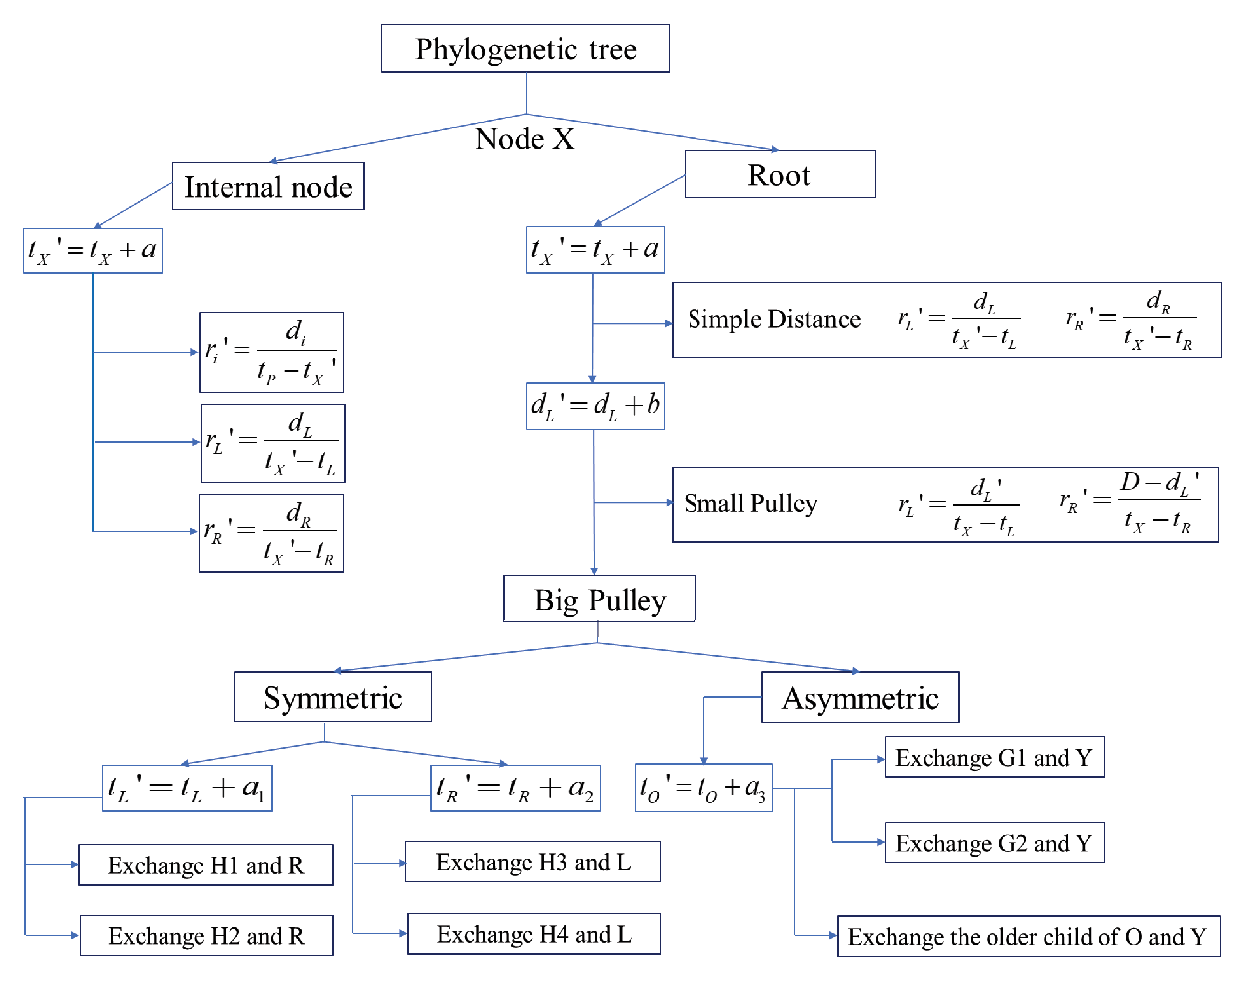
\includegraphics[width=12cm]{flowchart.eps}\\
\caption{\csentence{The flow chart of the constant distance operator.}
              }
\label{flowchart}
\end{figure}

\begin{figure}[h!]
\includegraphics[width=12cm]{internalnodes.eps}\\
\caption{\csentence{The illustration of operation on internal nodes.}
             The operator proposes a tree ${g_{in}}'$ based on tree $g_{in}$, during which $d_i$, $d_j$, $d_k$ are constant.}
\label{internalnodes}
\end{figure}

\begin{figure}[h!]
\includegraphics[width=12cm]{rootstrategy.eps}\\
\caption{\csentence{The operations of Simple Distance and Small Pulley.}
             Simple Distance proposes ${g_{r1}'}$ and keeps $d_i$, $d_x$ constant. Small Pulley proposes ${g_{r2}'}$ and ${d_i} + {d_x}$ remains constant.}
\label{simpledistance}
\end{figure}


\begin{figure}[h!]
\includegraphics[width=12cm]{exchangemethod.eps}\\
\caption{\csentence{The illustration of \textit{Exchange (\textbf{B},\textbf{ C})} method.}
             }
\label{exchangemethod}
\end{figure}

\begin{figure}[h!]
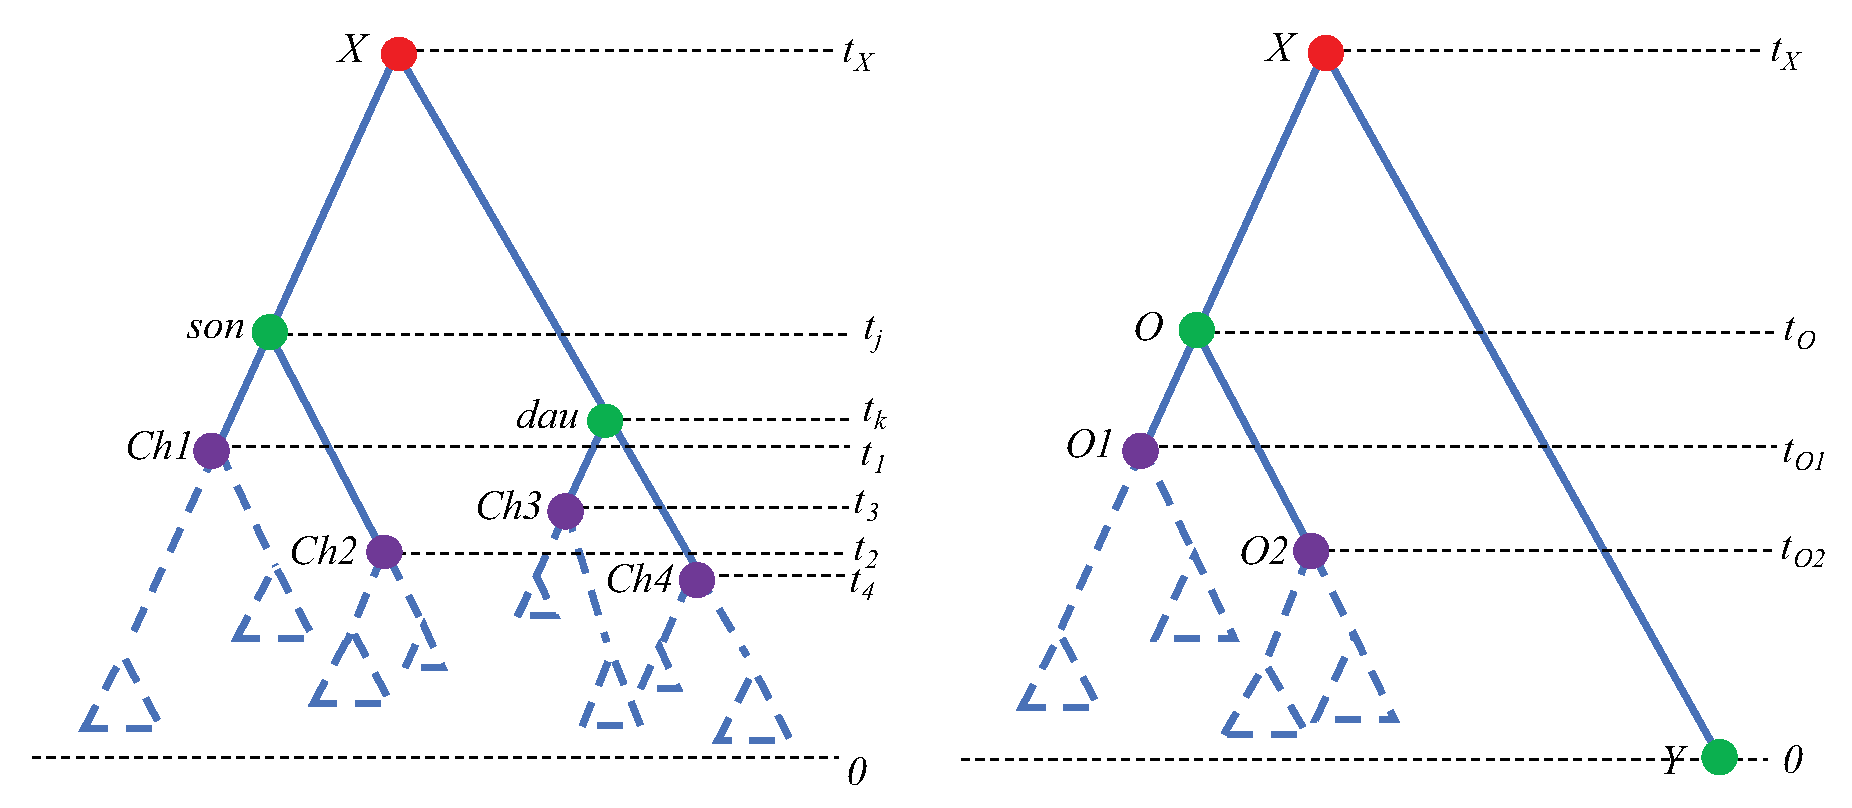
\includegraphics[width=12cm]{treeshape.eps}\\
\caption{\csentence{The illustration of tree shapes.}
             The symmetric tree is on the left and the asymmetric tree is on the right. The dashed triangles represent the potential subtrees rooted at the nodes.}
\label{treeshape}
\end{figure}

\begin{figure}[h!]
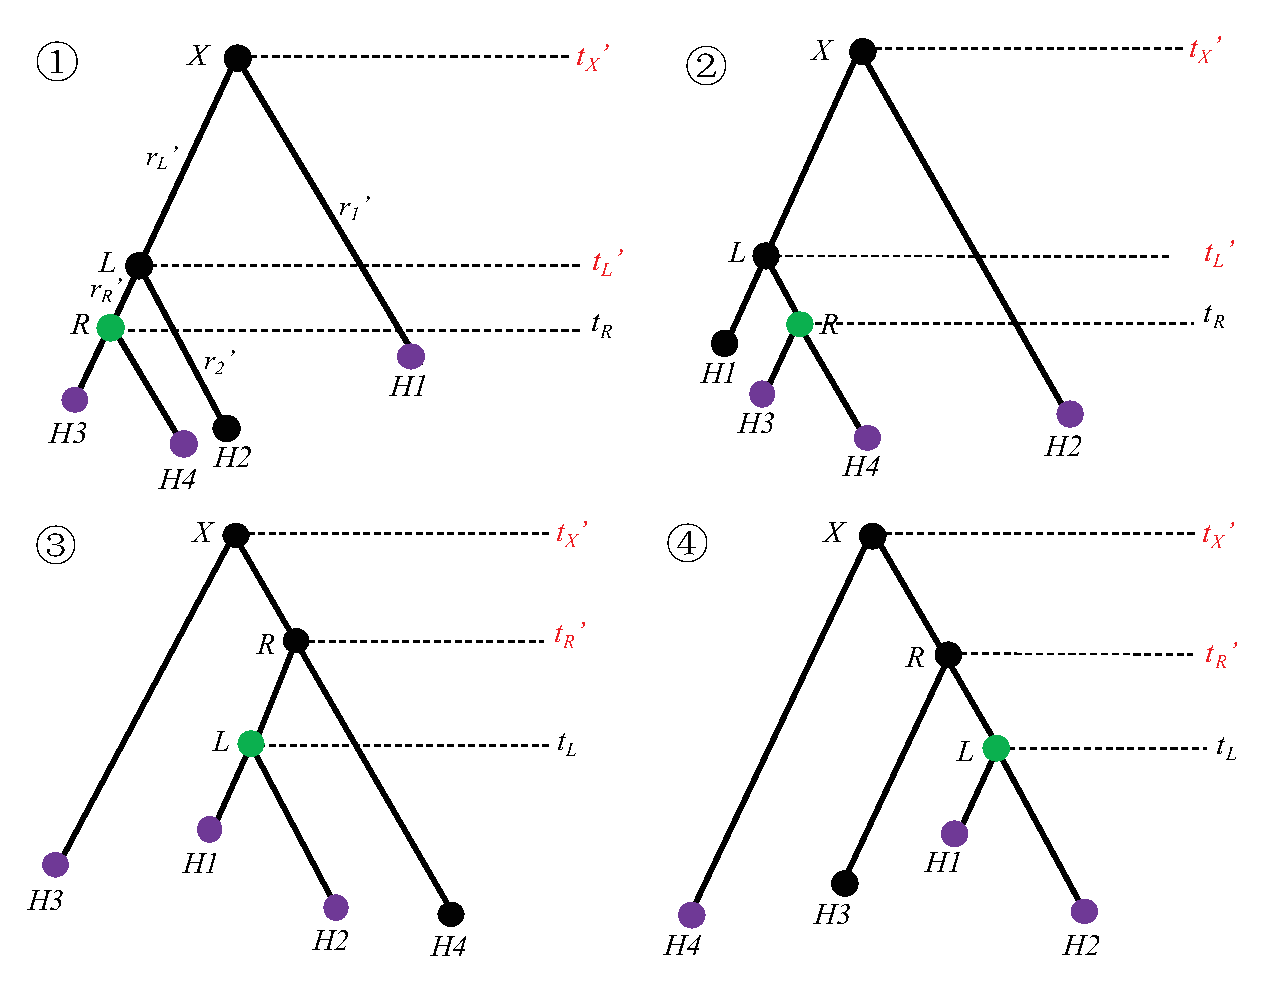
\includegraphics[width=12cm]{symmetric.eps}\\
\caption{\csentence{The illustration of symmetric trees.}
             }
\label{symmetric}
\end{figure}

\begin{figure}[h!]
\includegraphics[width=12cm]{asymmetric.eps}\\
\caption{\csentence{The illustration of asymmetric trees.}
             }
\label{asymmetric}
\end{figure}

\begin{figure}[h!]
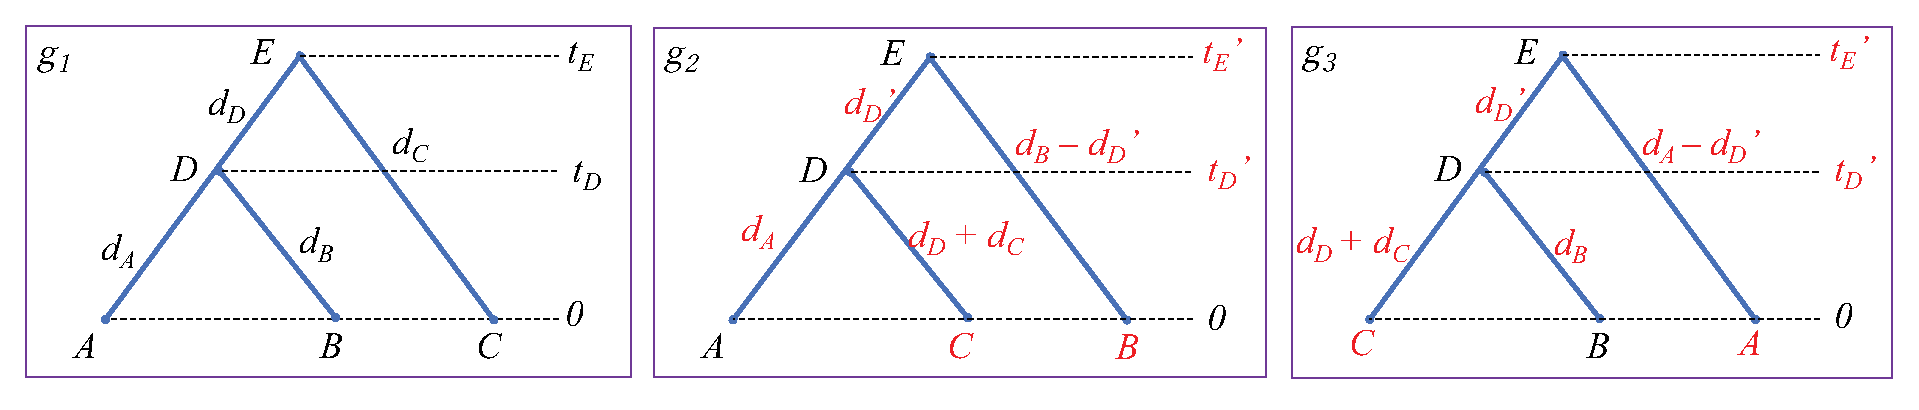
\includegraphics[width=12cm]{bigpulleyExp.eps}\\
\caption{\csentence{The illustration of sampling from prior.}
             }
\label{sampleprior}
\end{figure}

\begin{figure}[h!]
\centering
\subfigure[Senario 1: chain length = 10000000]{
\label{Fig.sub.1}
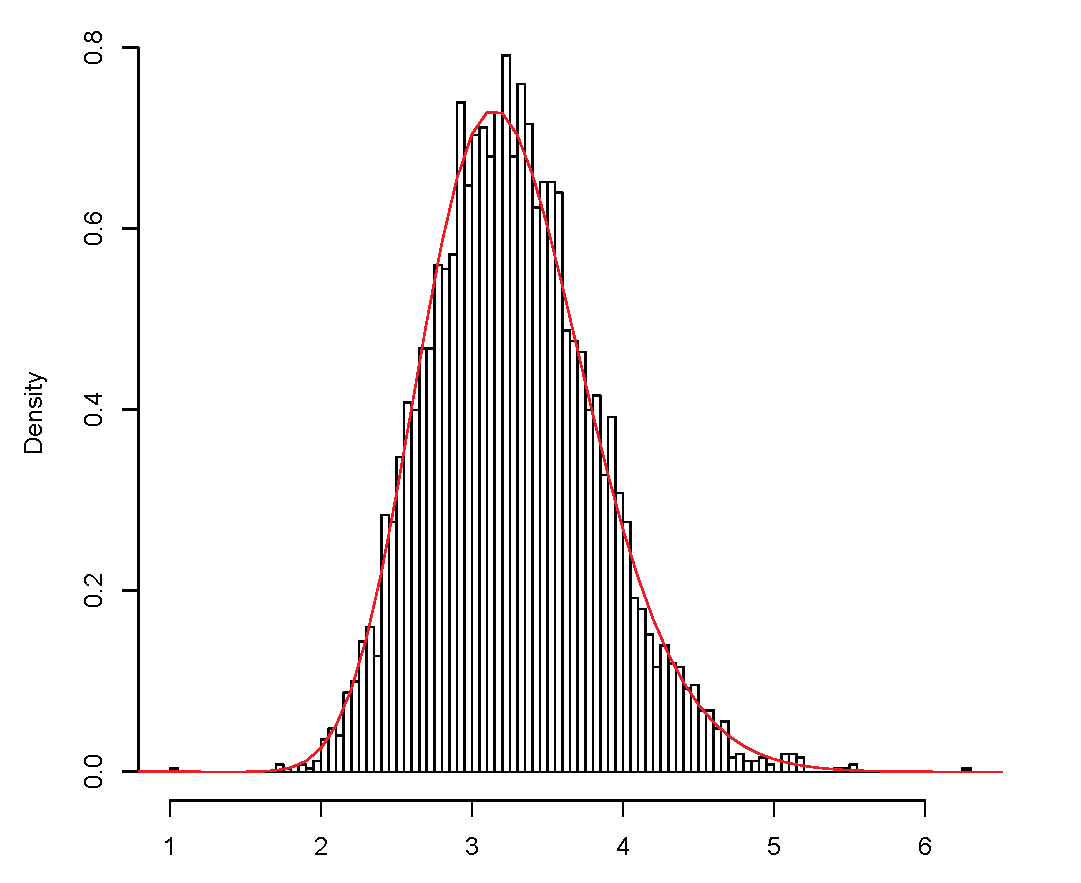
\includegraphics[width=0.45\textwidth]{Fig1}}
\subfigure[Senario 1: chain length = 20000000]{
\label{Fig.sub.2}
\includegraphics[width=0.45\textwidth]{Fig2}}
\subfigure[Senario 2: chain length = 10000000]{
\label{Fig.sub.3}
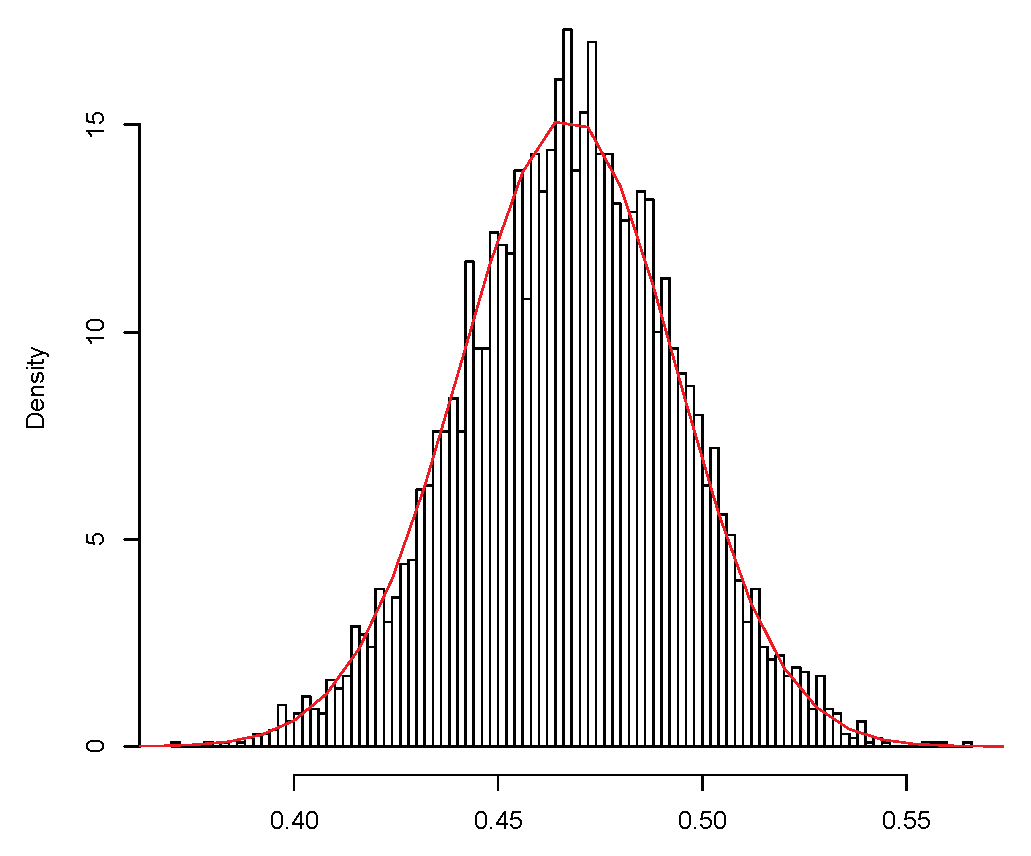
\includegraphics[width=0.45\textwidth]{Fig7}}
\subfigure[Senario 2: chain length = 20000000]{
\label{Fig.sub.4}
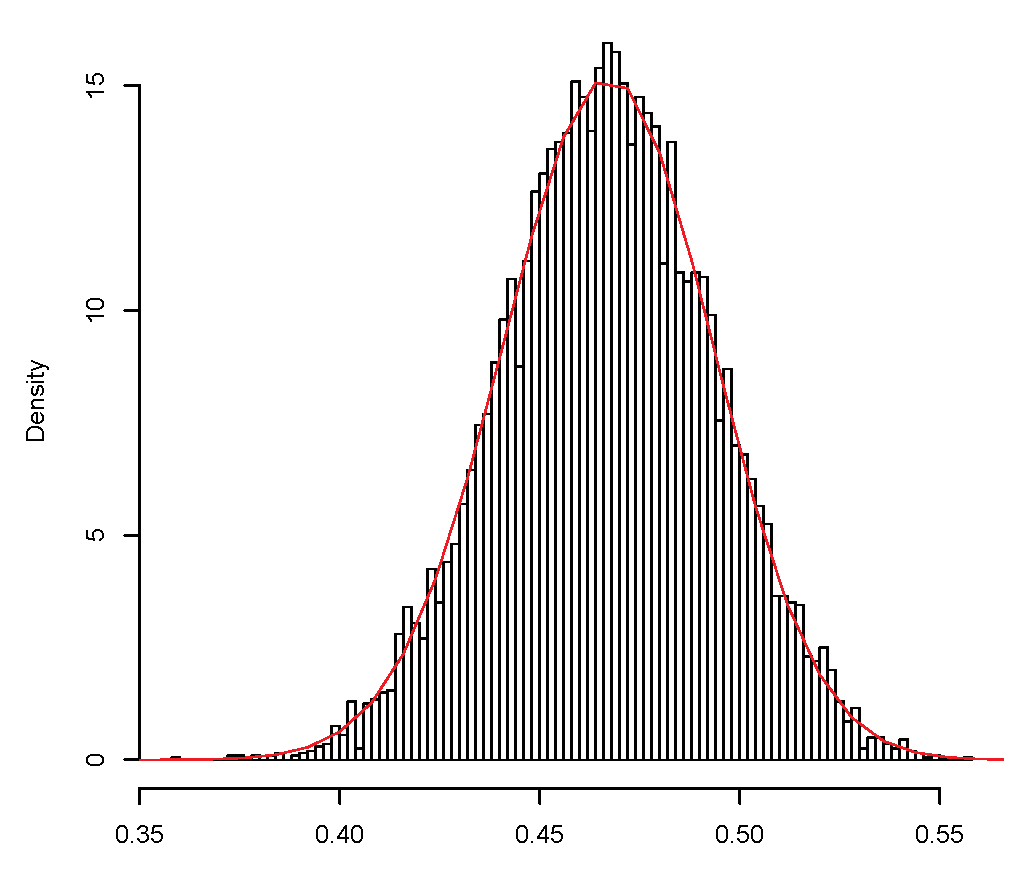
\includegraphics[width=0.45\textwidth]{Fig8}}
\caption{ Distributions of internal nodes}
\label{res_int}
\end{figure}

\begin{figure}[h!]
\centering
\subfigure[$t_E$ in Simple Distance]{
\label{Fig.sub.5}
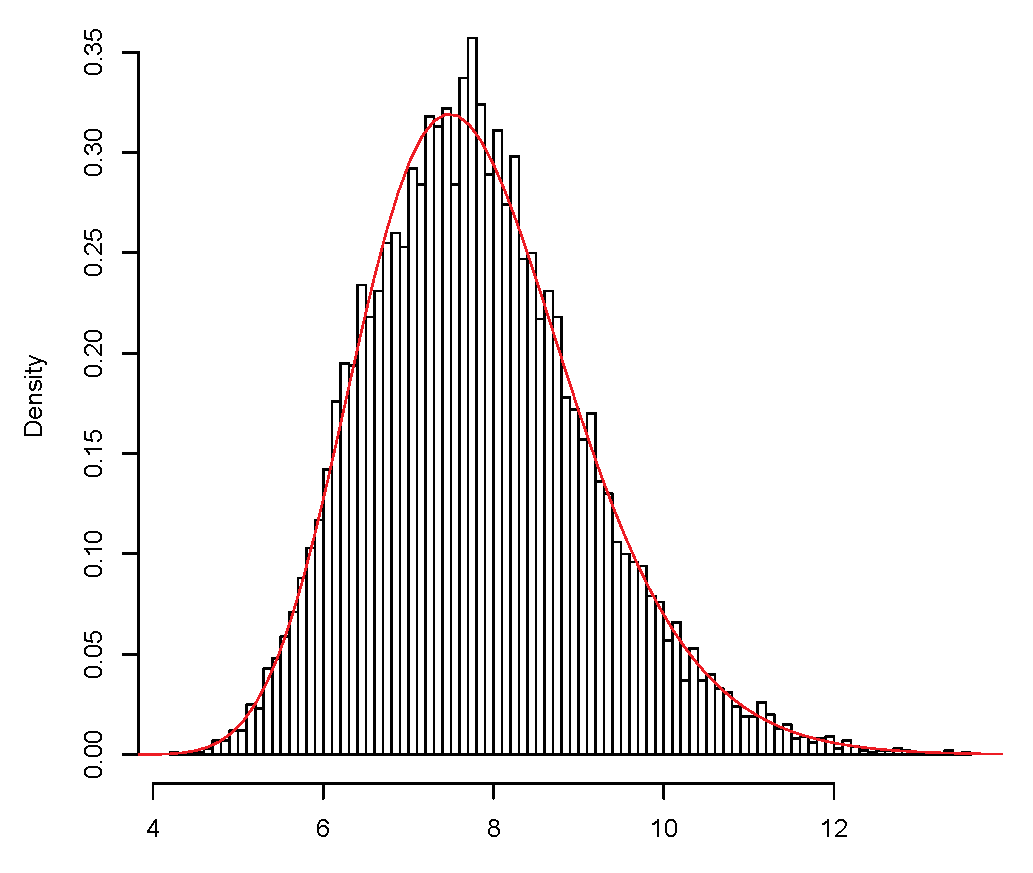
\includegraphics[width=0.35\textwidth]{RplotSD}}
\subfigure[$d_i$ in Small Pulley]{
\label{Fig.sub.6}
\includegraphics[width=0.35\textwidth]{RplotSP2}}
\subfigure[${d_i}$ in Big pulley]{
\label{Fig.sub.9}
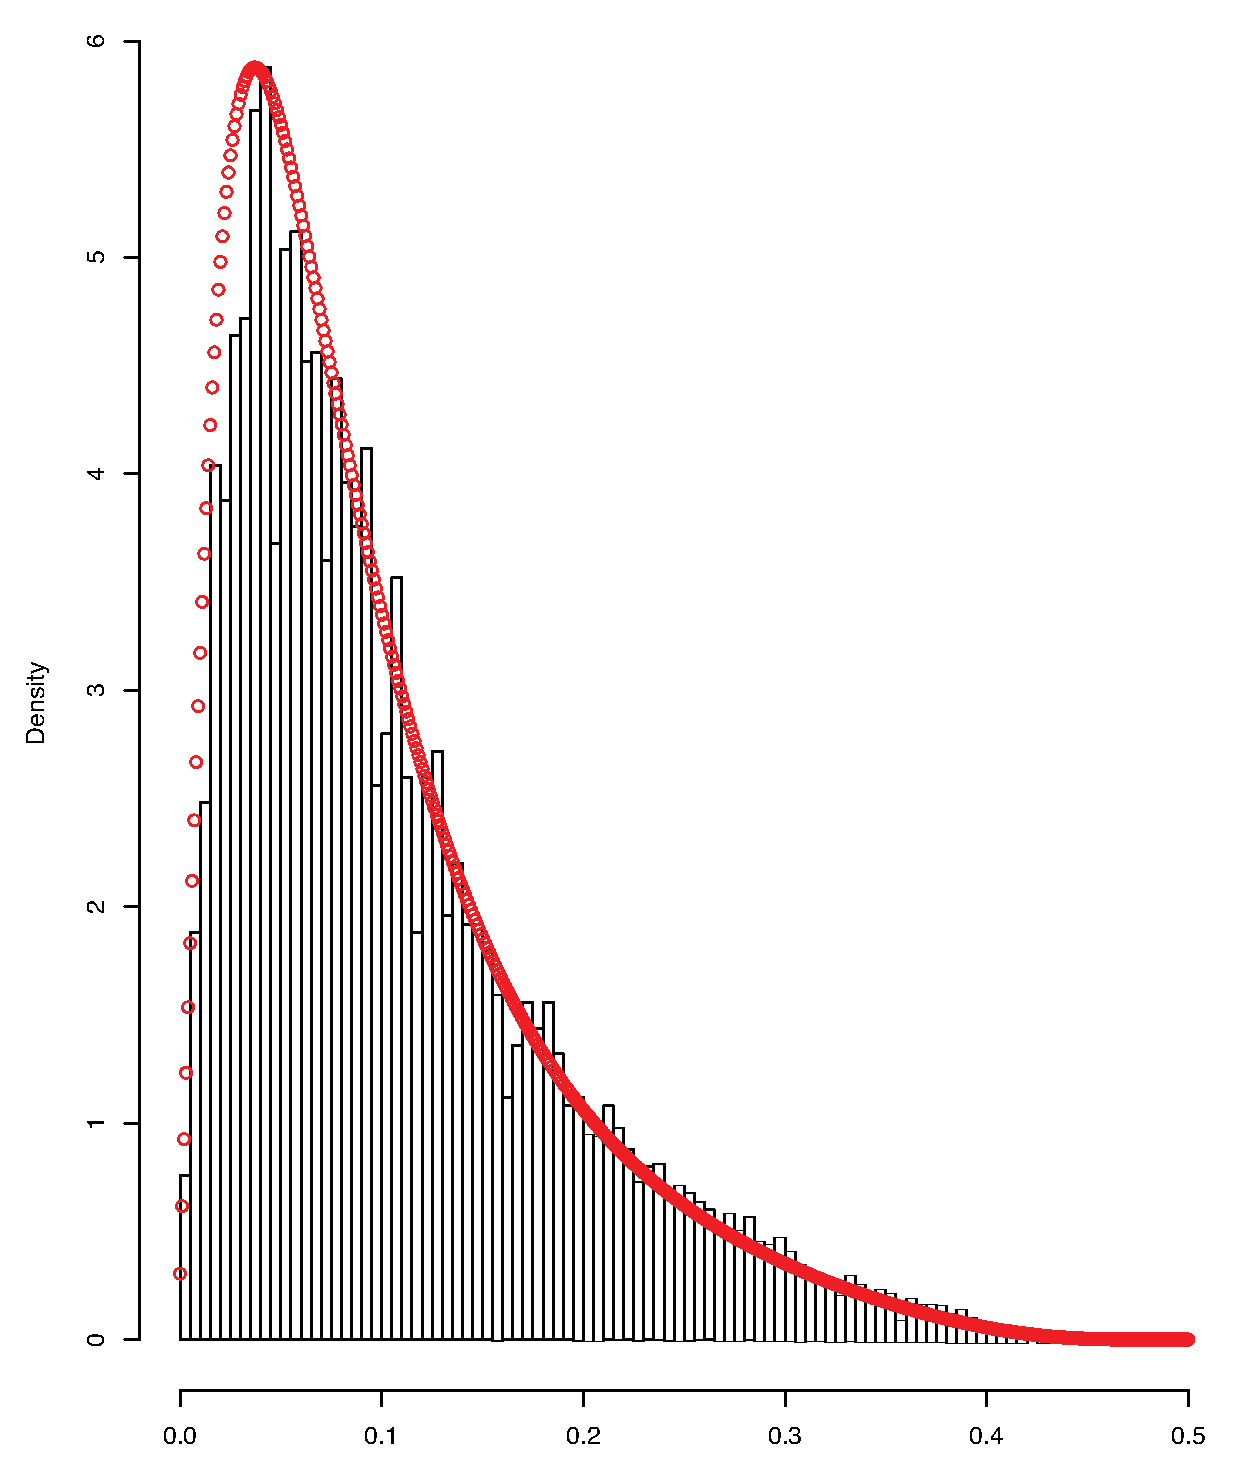
\includegraphics[width=0.35\textwidth]{bigd}}
\subfigure[${t_E}$ in Big pulley]{
\label{Fig.sub.10}
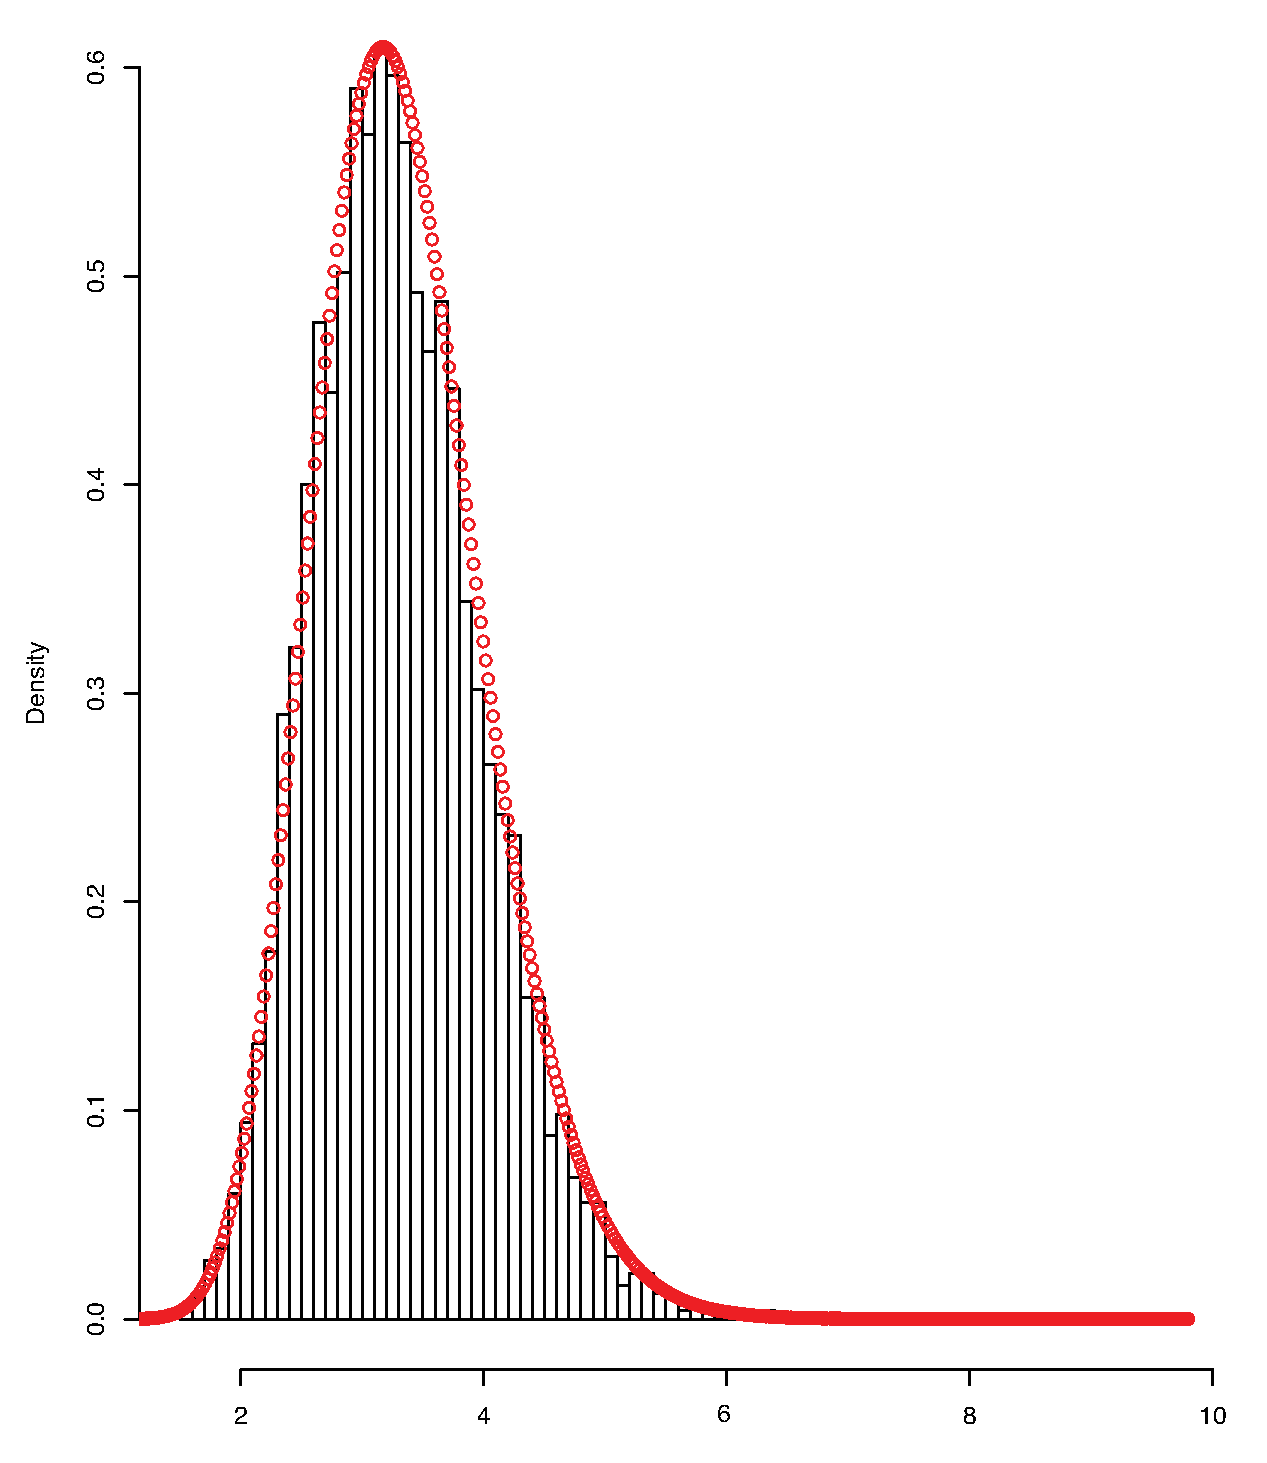
\includegraphics[width=0.35\textwidth]{bigT}}
\caption{Distributions of root}
\label{res_roo1}
\end{figure}

\begin{figure}[h!]
\includegraphics[width=12cm]{ModelValidation.eps}\\
\caption{\csentence{The models and prior distributions to simulate the sequence data.}
             }
\label{modelvalidation}
\end{figure}

\begin{figure}[h!]
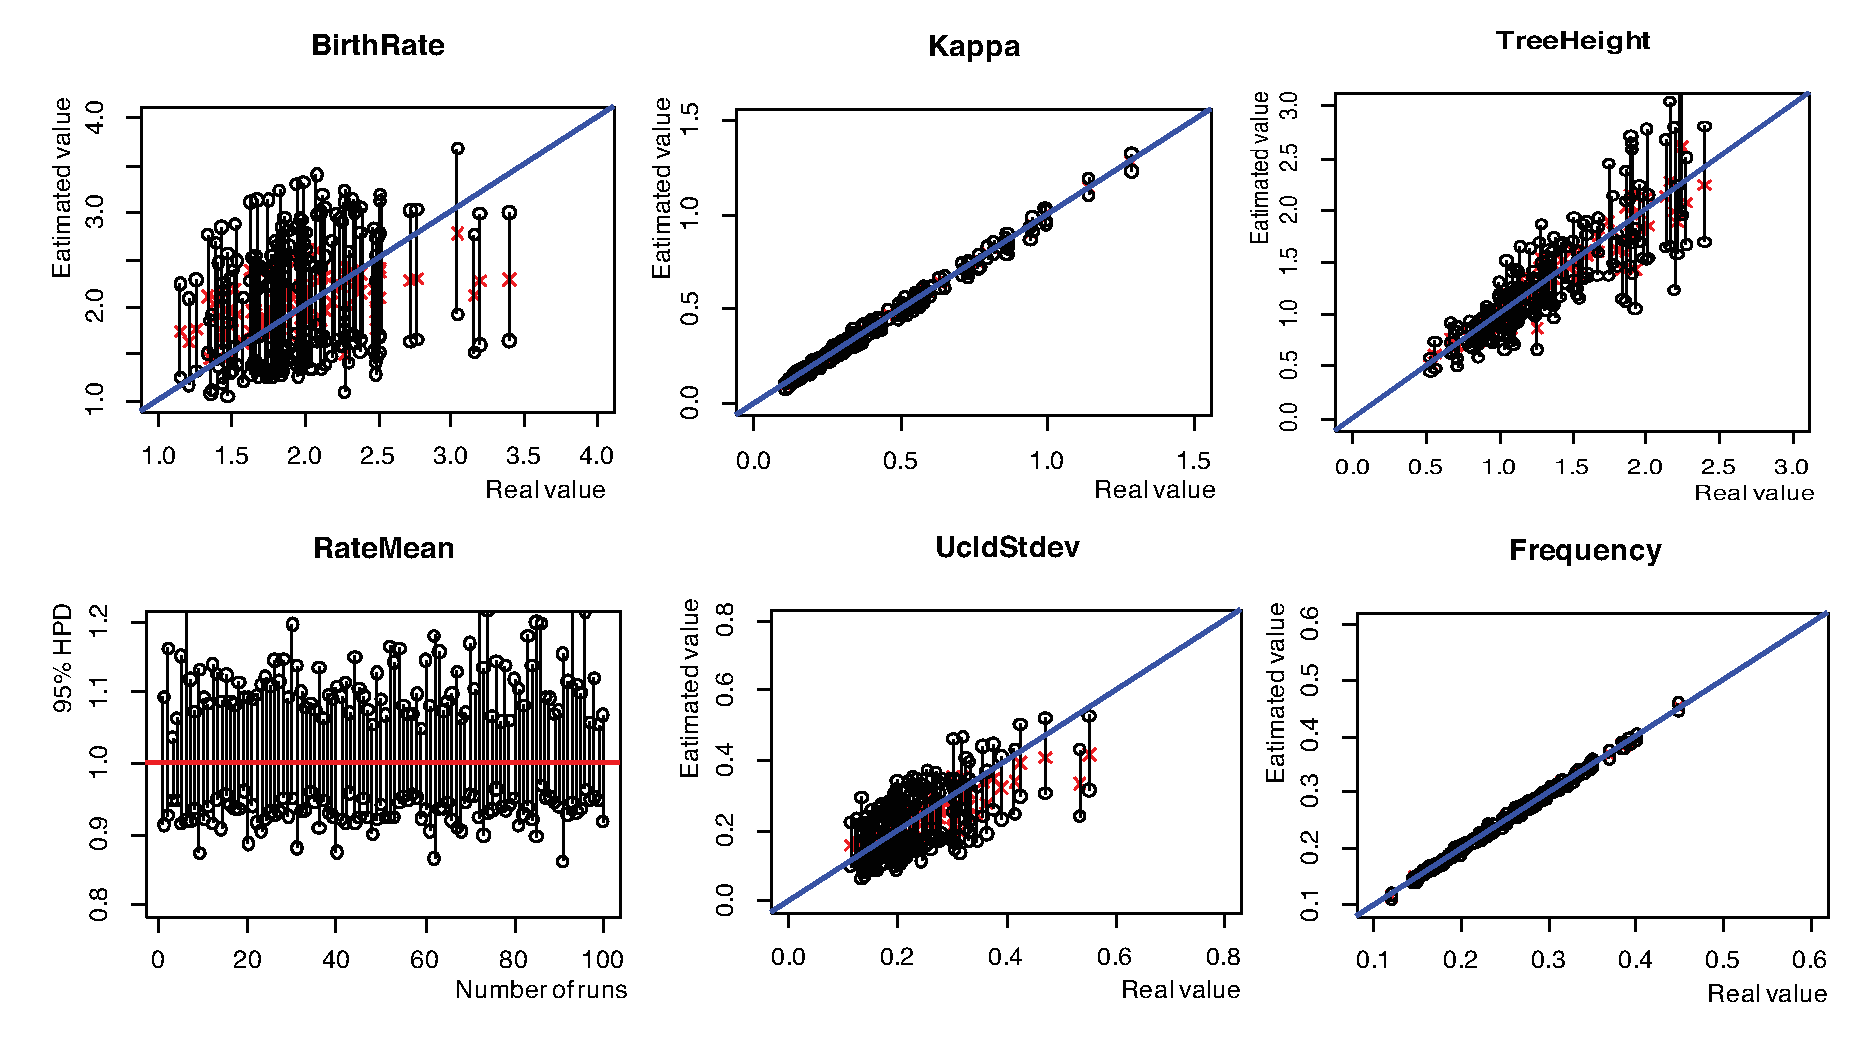
\includegraphics[width=12cm]{SmallTree.eps}\\
\caption{\csentence{Comparison of simulation study with 20 taxa.}
             }
\label{SmallTree}
\end{figure}

\begin{figure}[h!]
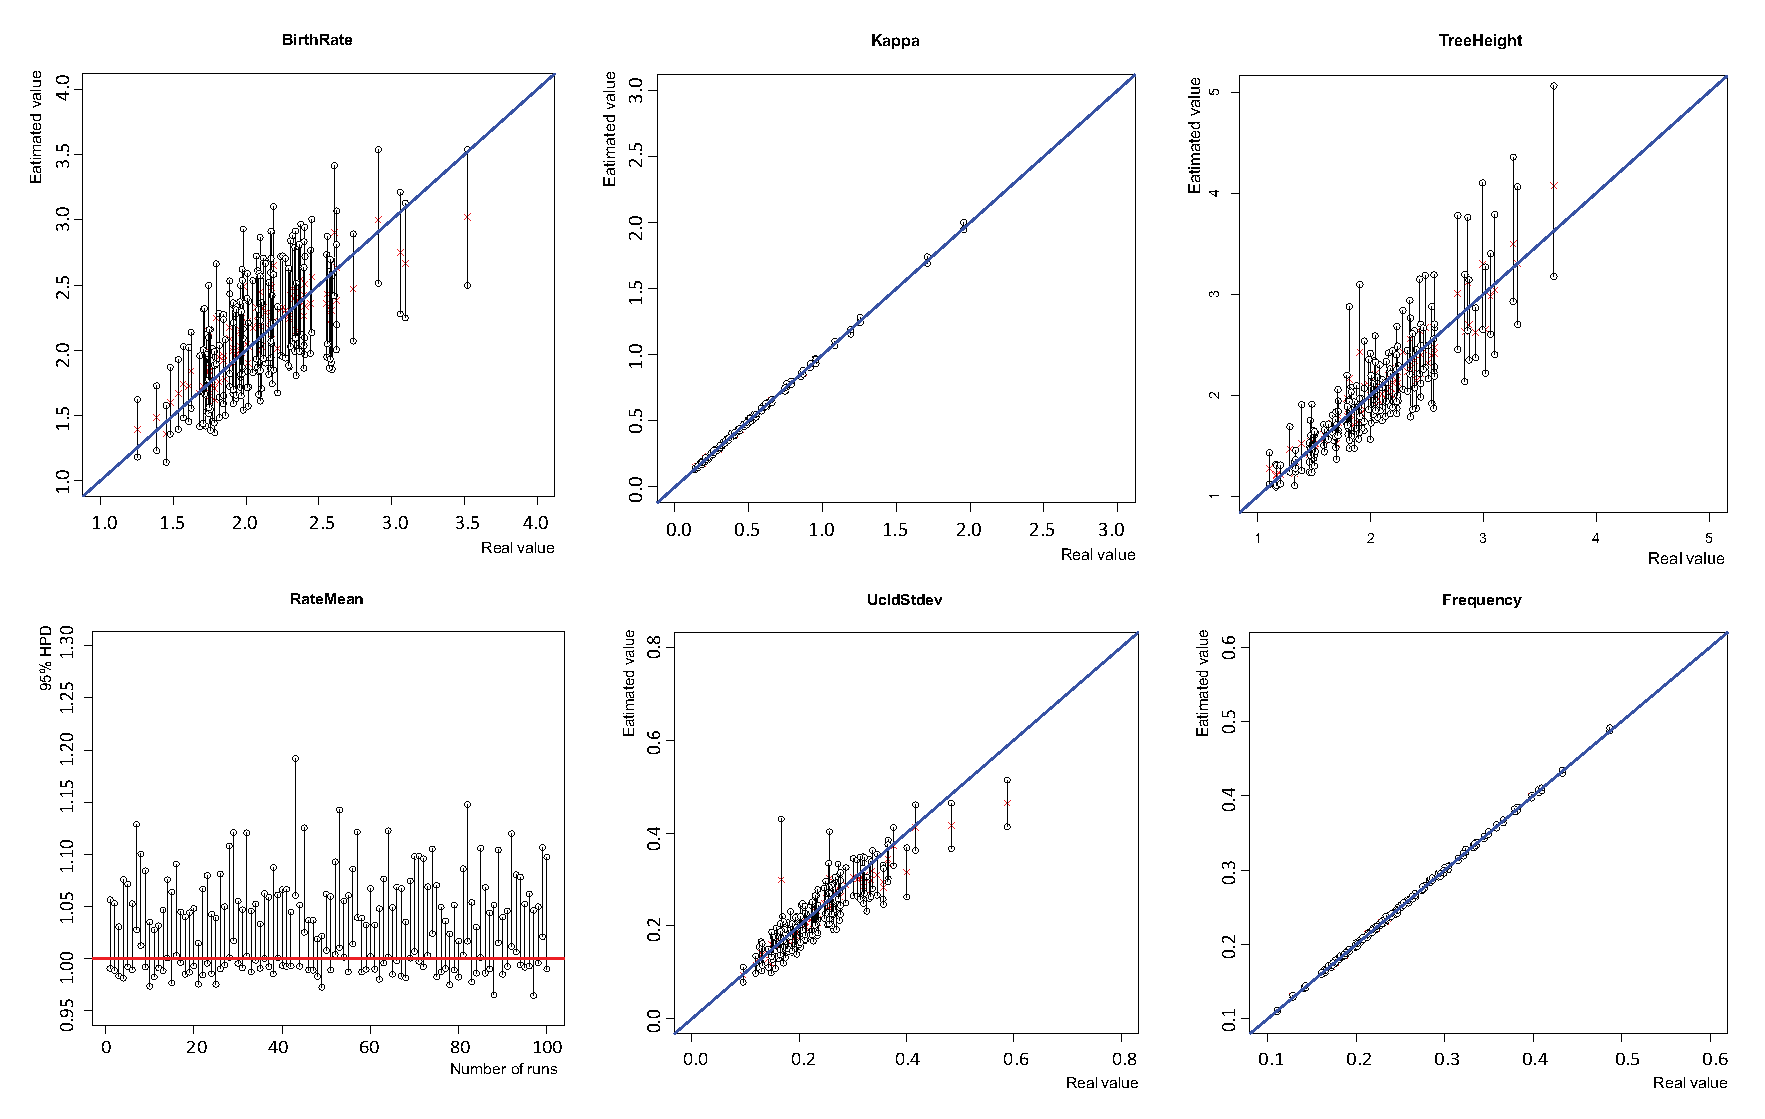
\includegraphics[width=12cm]{LargeTree.eps}\\
\caption{\csentence{Comparison of simulation study with 120 taxa.}
             }
\label{LargeTree}
\end{figure}

\begin{figure}[h!]
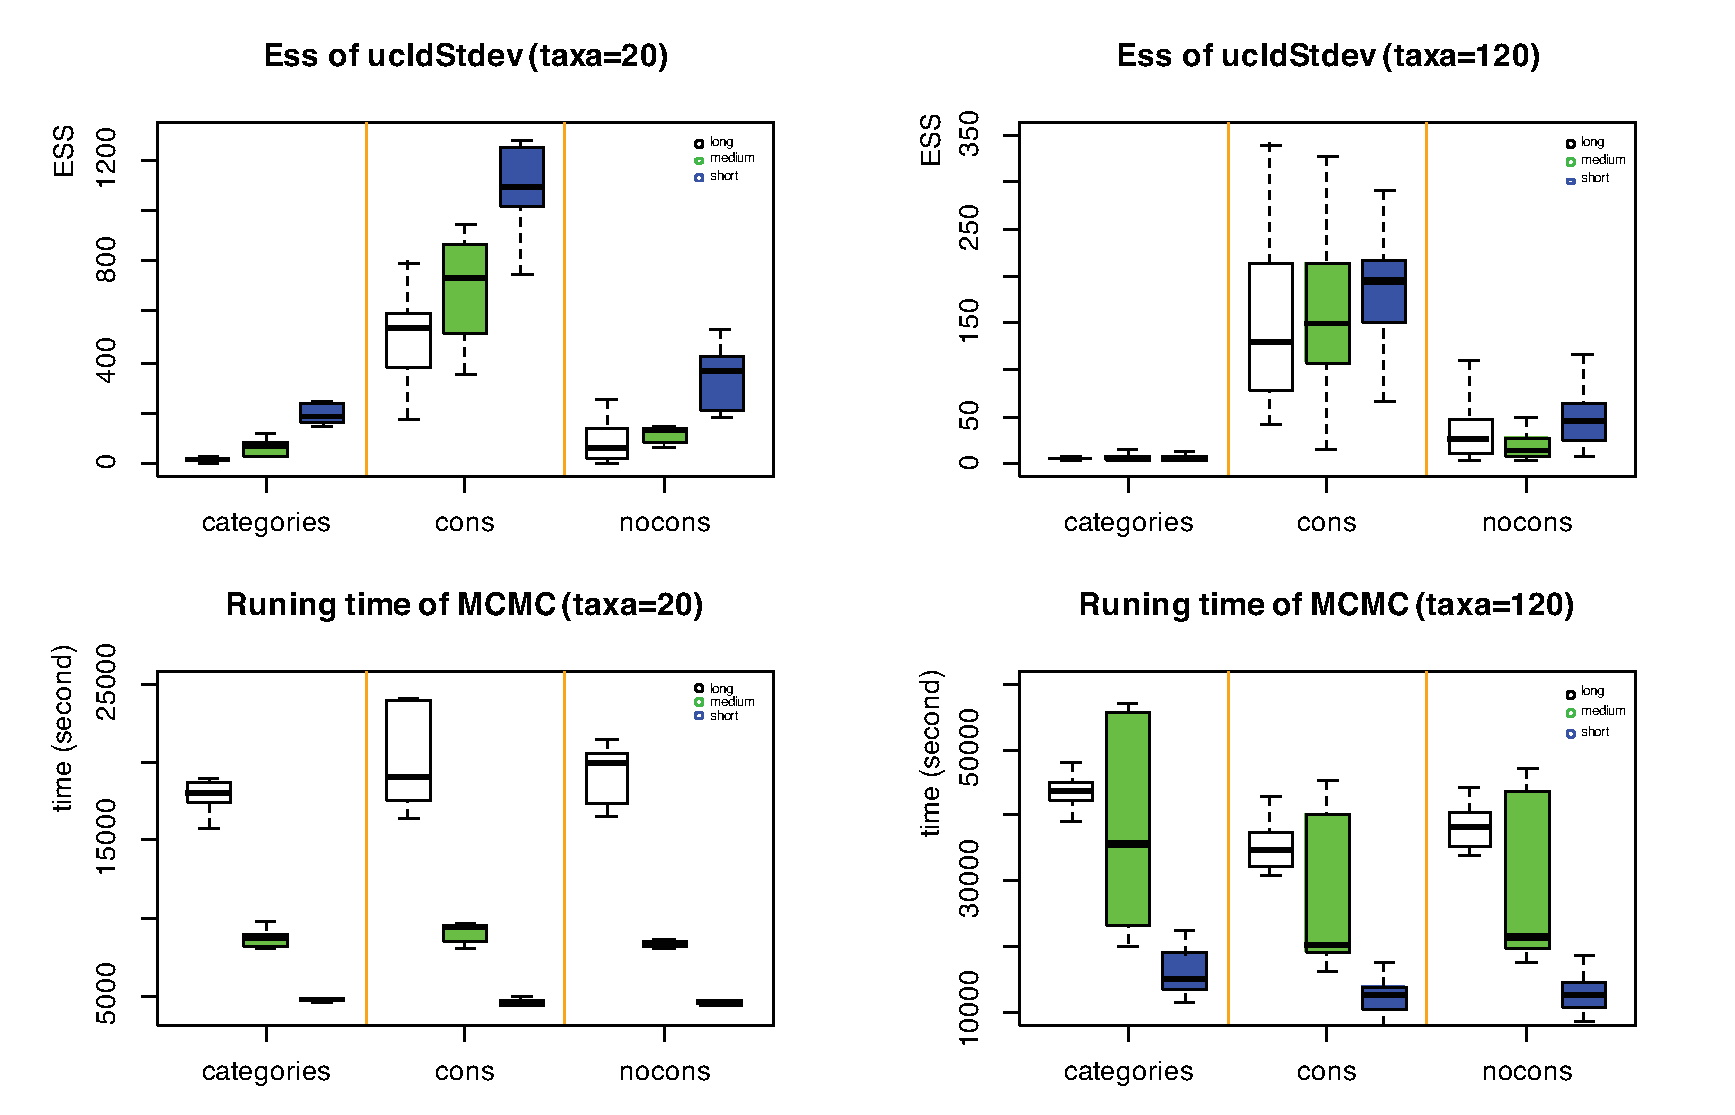
\includegraphics[width=12cm]{Efficiency.eps}\\
\caption{\csentence{Comparison of ESS and running time using simulated data.}
             }
\label{eff_comp}
\end{figure}

\begin{figure}[h!]
\centering
\subfigure{
\label{P_run}
\includegraphics[width=0.5\textwidth]{primates1.eps}}
\subfigure{
\label{P_ess}
\includegraphics[width=0.5\textwidth]{primates2.eps}}
\caption{Comparison the ESS and ESS using primates data}
\label{eff_comp2}
\end{figure}

\begin{figure}[h!]
\centering
\subfigure[Unrooted tree]{
\label{Fig.sub.11}
\includegraphics[width=0.4\textwidth]{unrootedtree}}
\subfigure[Rooted time tree]{
\label{Fig.sub.12}
\includegraphics[width=0.4\textwidth]{initialtree}}
\caption{Initialising the rooted time tree based on an unrooted tree}
\label{withoutdata}
\end{figure}

\begin{figure}[h!]
\centering
\subfigure[Uncertainties in summary tree]{
\label{summary3}
\includegraphics[width=0.4\textwidth]{summary3}}
\subfigure[Ratite phylogeography \cite{cooper2001complete}]{
\label{ratites}
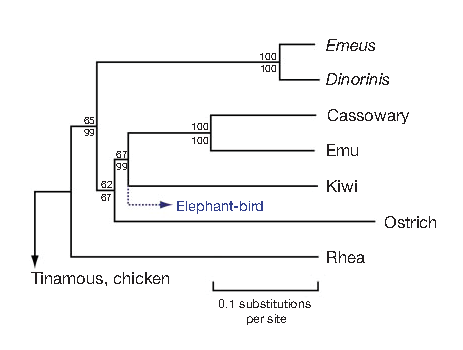
\includegraphics[width=0.4\textwidth]{ratites}}
\caption{Comparison of ratites phylogenetic trees}
\label{fixedtree}
\end{figure}

\begin{figure}[h!]
\includegraphics[width=12cm]{rateandtime.eps}\\
\caption{\csentence{Correlation between rates and times in the ratites tree.}
             }
\label{correlation}
\end{figure}
%%%%%%%%%%%%%%%%%%%%%%%%%%%%%%%%%%%
%%                               %%
%% Tables                        %%
%%                               %%
%%%%%%%%%%%%%%%%%%%%%%%%%%%%%%%%%%%
%% Use of \listoftables is discouraged.
%%
\section*{Tables}
\begin{table}[h!]
  \centering
\begin{tabular}{c|cccc|c|c|cccc}
  \hline
&\multicolumn{4}{c|}{genetic distances (fixed)}&$t_D$&$t_E$&\multicolumn{4}{c}{initial rates}\\
&${d_j}$&${d_k}$&${d_x}$&${d_i}$&initial&(fixed)&${r_j}$&${r_k}$&${r_x}$&${r_i}$\\
\hline
Scenario 1&0.1&0.2&0.4&0.27&1&10&0.1&0.2&0.04&0.03\\
\hline
Scenario 2&0.4&0.8&2.4&1.6&0.4&0.8&1&2&3&4\\
  \hline
\end{tabular}
\caption{Initial settings for internal nodes}\label{ini_inter}
\end{table}

\begin{table}[h!]
  \centering
\begin{tabular}{c|c|ccc|ccc|c}
  \hline
&\multirow{2}*{Chain Length}&\multicolumn{3}{c|}{Sample from MCMC}&\multicolumn{3}{c|}{R curve}&Plot\\
&~&Mean&Err&StdEv&Mean&Err&StdEv&\\
\hline
\multirow{2}*{Senario 1}&10000000&3.2727&8.3e-3&0.5467&\multirow{2}*{3.2669}&\multirow{2}*{1.3e-06}&\multirow{2}*{0.5553}&Fig.\ref{Fig.sub.1}\\
~&20000000&3.271&6.1e-3&0.5616&~&~&~&Fig.\ref{Fig.sub.2}\\
\hline
\multirow{2}*{Senario 2}&10000000&0.4677&3.9e-04&0.0265&\multirow{2}*{0.4667}&\multirow{2}*{3.5e-05}&\multirow{2}*{0.0262}&Fig.\ref{Fig.sub.3}\\
~&20000000&0.4672&2.8e-04&0.0262&~&~&~&Fig.\ref{Fig.sub.4}\\
  \hline
\end{tabular}
\caption{Results of internal nodes}\label{res_inter}
\end{table}

\begin{table}[h!]
  \centering
\begin{tabular}{c|cccc|c|c|cccc}
  \hline
\multirow{2}*{strategy}&\multicolumn{4}{c|}{genetic distances}&\multirow{2}*{$t_D$}&\multirow{2}*{$t_E$}&\multicolumn{4}{c}{initial rates}\\
~&${d_j}$&${d_k}$&${d_x}$&${d_i}$&~&~&${r_j}$&${r_k}$&${r_x}$&${r_i}$\\
\hline
Simple distance&0.1&0.2&0.4&0.27&1&10&0.1&0.2&0.04&0.03\\
Small pulley&0.1&0.2&\multicolumn{2}{|c|}{0.67}&1&10&0.1&0.2&0.04&0.03\\
Big pulley&0.5&0.5&\multicolumn{2}{|c|}{0.5}&5&10&0.1&0.1&0.03&0.04\\
  \hline
\end{tabular}
\caption{Initial settings for simple distance}\label{ini_sim}
\end{table}

\begin{table}[h!]
\centering
\begin{tabular}{c|c|cc|cc|cc}
  \hline
\multirow{2}*{Strategy}&\multirow{2}*{Variable}&\multicolumn{2}{c|}{Sample from MCMC}&\multicolumn{2}{c|}{R curve}&\multirow{2}*{Plot}\\
&~&Mean&StdEv&Mean&StdEv&\\
\hline
Simple distance&$t_E$&7.8081&1.2884&7.818691&1.299236&Fig.\ref{Fig.sub.5}\\
\hline
Small Pulley&${d_i}$&0.3480&0.0492&0.3476&0.0494&Fig.\ref{Fig.sub.6}\\
\hline
\multirow{2}*{Big Pulley}&${d_i}$&0.1016&0.0766&0.0960&0.0760&Fig.\ref{Fig.sub.9}\\
~&$t_E$&3.3017&0.6908&3.3095&0.6912&Fig.\ref{Fig.sub.10}\\
\hline
\end{tabular}
\caption{Results for root}\label{res_sma}
\end{table}

\begin{table}[h!]
  \centering
\begin{tabular}{cccccccc}
\hline
&BirthRate&TreeHeight&RateMean&UcldStdev&Kappa&Frequency\\
\hline
20 taxa&93&98&100&95&100&100\\
120 taxa&100&98&85&94&100&100\\
\hline
\end{tabular}
\caption{Number of real values lying in the 95\% HPD}\label{num_hpd}
\end{table}

\begin{table}[h!]
  \centering
\begin{tabular}{cc|cc|cc}
\hline
&&\multicolumn{2}{c|}{ESS}&\multicolumn{2}{c}{Running time}\\
\hline
&Length&20 taxa&120 taxa&20 taxa&120 taxa\\
categories&20000&13&4&18635&44155\\
&10000&58&6&8660&36406\\
&5000&171&8&4690&15956\\
Average&&81&6&10662&32172\\
\hline
cons&20000&616&147&20207&35406\\
&10000&646&161&8967&25589\\
&5000&993&186&4581&12487\\
Average&&752&165&11252&24494\\
\hline
nocons&20000&86&63&19344&38245\\
&10000&153&20&8361&30521\\
&5000&296&48&4499&12940\\
Average&&179&43&10735&27236\\
\hline
\end{tabular}
\caption{Results of ESS and running time}\label{eff_comp1}
\end{table}
%%%%%%%%%%%%%%%%%%%%%%%%%%%%%%%%%%%
%%                               %%
%% Additional Files              %%
%%                               %%
%%%%%%%%%%%%%%%%%%%%%%%%%%%%%%%%%%%

%\section*{Additional Files}
%  \subsection*{Additional file 1 --- Sample additional file title}
%    Additional file descriptions text (including details of how to
%    view the file, if it is in a non-standard format or the file extension).  This might
%    refer to a multi-page table or a figure.
%
%  \subsection*{Additional file 2 --- Sample additional file title}
%    Additional file descriptions text.


\end{backmatter}
\end{document}
